\documentclass[12pt, a4paper]{report}
\usepackage[russianb]{babel}
\usepackage{graphics}
%\usepackage[pdftex]{graphicx}
\parindent 0.5cm
\textwidth 15.5cm \textheight 24cm \topmargin -1.5cm
\evensidemargin .5cm \oddsidemargin .5cm \baselineskip=14pt plus
1pt

\newtheorem{prope}{Свойство} [chapter]

\begin{document}
\begin{flushright}
\today
\tableofcontents
\end{flushright}

\chapter {Обратная спектральная задача. Метод модифицированных моментов.}
Рассмотрим набор позитивных борелевских мер
$\mu_1,\mu_2,\ldots,\mu_p$ с бесконечно большим количеством точек
роста на соответствующих носителях
$\Delta_j, j=1,...p$. \\
Введем мульти-индекс $\bf n \rm$ $=(n_1,\ldots,n_p)$ и рассмотрим \it совместно ортогональные многочлены \rm, такие что
$$
\int Q_{ \bf n \rm } (x) x^{\upsilon} d\mu_k(x) = 0, \hspace{1cm} \upsilon = 0,1,... n_k-1, k = 1, ... p 
$$
$$\mbox{deg} Q_{ \bf n \rm} \leq n := \sum\limits_{k=1}^{p} n_k$$
В общем случае совместно ортогональные многочлены существуют для любого мульти-индекса, но определены неоднозначно. \\
При \it условии нормальности \rm мульти индекса $\mbox{deg}Q_n=n$ совместно ортогональные многочлены уникальны с точностью до константы. \\
Пусть для определенности $Q_n$ обозначают многочлены со старшим коэффициентом равным единице. Ограничим множество мульти-индексов условием:
$$\bf n \rm =(\underbrace{k+1,\ldots,k+1}_{d},\underbrace{k,\ldots,k}_{p-d}),$$ $$k\in{\mbox{Z}}_{+},n=pk+d $$
При условии нормальности все таких индексов совместно ортогональные многочлены удовлетворяют следующим реккурентным соотношениям:
$$
Q_{-p}=\ldots=Q_{-1}=0, \hspace{1cm} Q_0=1,
$$
$$
Q_{n+1}=(x+a_{n,n})Q_n+a_{n,n-1}Q_{n-1}+\ldots + a_{n,n-p}Q_{n-p}
$$
Рассмотрим $p+2$ диагональную полубесконечную матрицу $A$, составленную из коэффициентов реккурентных соотношений:
$$
A= \left(\begin{array}{ccccccc}
a_{0,0}&a_{0,1}&0&0&0&0&\cdots\\
a_{1,0}&a_{1,1}&a_{1,2}&0&0&0&\cdots\\
\cdots&\cdots&\cdots&\cdots&\cdots&\cdots&\cdots\\
a_{p,0}&a_{p,1}&a_{p,2}&\cdots&a_{p,p+1}&0&\cdots\\
0&a_{p+1,1}&a_{p+1,2}&\cdots&a_{p+1,p+1}&a_{p+1,p+2}&\cdots\\
\cdots&\cdots&\cdots&\cdots&\cdots&\cdots&\cdots
\end{array}\right)
$$  
с условиями, что:
$$a_{n,n-p}\not=0,\ldots,a_{n,n+1}\not=0, \hspace{1cm} a_{i,j}=0, j>i+1,i>j+p $$
Матрица $A$ задает разностный оператор $A$ в пространстве $l^2 (\sf \bf N \rm)$ \\
Пусть $\{ e_n \}_{0}^{\infty}$ cтандартный базис в $l^2$.   
Оператор $A$ определен как
$$
Ae0=a_{0,0}e_0+ a_{1,0}e_1 + \ldots + a_{p,0}e_p
$$
$$
Ae_k=a_{k-1,k}e_{k-1}+a_{k,k}e_{k}+\ldots+a_{k+p,k}e_{k+p}, \hspace {0.5cm} k\geq 1
$$
Функций $(f_1, ... , f_p)$ называются \it резольвентными \rm или \it функциями Вейля \rm оператора $A$ 
$$
f_j(z) := \left(\frac {e_{j-1}} {(zI - A)}, e_0 \right)
$$
Если оператор $A$ ограничен $\mbox{sup}_{i,j} \vert a_{i,j} \vert < \infty $ то резольвентные функции можно разложить в степенные ряды в бесконечности.
$$
f_j(z) = \sum\limits_{k=0}^{\infty}{\frac{(A^k e_{j-1}, e_0)}{z^{k+1}}}, \hspace{0.5cm} \vert z \vert > \Vert A \Vert, j=1,\ldots,p
$$
Для $j=1,\ldots p$ 
$$
s_k :=(A^k e_{j-1}, e_0)
$$ 
называются \it моментами \rm оператора $A$, а множество $\{e_0, \ldots e_{p-1}\}$ - \it циклическим множеством \rm оператора $A$ \\
Спектральные свойства оператора $A$ тесно связаны с асимптотическими свойствами совместно ортогональных многочленов. \\
Резольвентные функции и моменты связаны с борелевскими мерами которые называют в данном контексте \it спектральными мерами \rm оператора:
$$
f_j(z) = \int _{\Delta_j} \frac{d\mu_j(x)}{z-x}, \hspace{0.5cm} s_n^{(j)}=\int \limits_{\Delta_j} {z^n d\mu_j (z)}
$$
\bf Прямая спектральная задача \rm состоит определении элементов матрицы оператора по заданному набору спектральных мер. \\
\bf Обратная спектральная задача \rm состоит в восстановлении оператора по набору его спектральных мер. \\
В общем случае обратная спектральная задача плохо обусловлена. \\
Цель численных экспериментов в этой главе проверить рассмотреть некоторые стандартные системы мер и проверить утверждение, что \ldots являются \it компактным возмущением \rm некоторого референс-оператора.

\newpage 
\subsection{Системы Стилтьеса}
Рассмотрим совместно ортогональные многочлены удовлетворяющие следующему реккурентному соотношению:
$$
Q_{n+1}=zQ_n+ a_{n,n-p}Q_{n-p}
$$
При $a_j=1$ случай является обощением полиномов Чебышева 2го рода \\
Соответствующий оператор выражен матрицей
\begin{equation}
L = \left(\begin{array}{ccccccc}
0 & 1&0&0&0&0&\cdots\\
0 & 0 &1&0&0&0&\cdots\\
\cdots&\cdots&\cdots&\cdots&\cdots&\cdots&\cdots\\
a_0&0&0&\cdots&1&0&\cdots\\
0&a_1&0&\cdots&0&1&\cdots\\
\cdots&\cdots&\cdots&\cdots&\cdots&\cdots&\cdots
\end{array}\right)
\end{equation}

\begin{prope}
Если для всех $n$ выполняется условие $a_n > 0$ тогда существует система положительных мер $\mu_j, j=1,\ldots,p$ с общим носителем $[0, \infty)$. 
\end{prope}
Соответствующие резольвентные функции 
$$
S_j(z) = \int \limits_{0}^{\infty} {\displaystyle\frac{d\mu_j(x)}{z-x}}, \hspace{0.5cm} j=1, \ldots p
$$
называют \it функциями Стильтеса\rm.
\begin{prope}
При $a_n > 0, n \geq 1$ оператор $L$ ограничен тогда и только тогда, когда общий носитель мер $\mu_j$ является ограниченным множеством
\end{prope}
\begin{prope}
Соответствующие спектральные меры $\mu_1, \ldots, \mu_p$ оператора $L$ абсолютно непрерывны на носителе $S_0$, который представлен звездоподобным множеством на комплексной плоскости, лучи которого образованы $p+1$ отрезками:
$$
[0,\alpha], [0, \alpha e^{2\pi i / (p+1)}], \ldots , [0, \alpha e^{p 2\pi i /(p+1)}]
$$ 
где $\alpha=\displaystyle \frac{p+1}{p^{p/(p+1)}}$
\end{prope}
\begin{prope}
Любой оператор $L$ при условии $\lim \limits_{k \rightarrow \infty} a_n = 1$ является компактным возмущением референсного оператора
 \begin{equation}
L_0 = \left(\begin{array}{ccccccc}
0 & 1&0&0&0&0&\cdots\\
0 & 0 &1&0&0&0&\cdots\\
\cdots&\cdots&\cdots&\cdots&\cdots&\cdots&\cdots\\
1&0&0&\cdots&1&0&\cdots\\
0&1&0&\cdots&0&1&\cdots\\
\cdots&\cdots&\cdots&\cdots&\cdots&\cdots&\cdots
\end{array}\right)
\end{equation}
\end{prope}


\newpage
\subsection {Система Стилтьеса $p=2, a_j=1$}
Система представлена мерами $\mu^0_1, \mu^0_2$ непрерывными на множестве $S_0$ состоящем из 3 отрезков на комплексной плоскости:
$$
[0, \displaystyle \frac{3}{2} \sqrt[3]{2}], [0, \displaystyle \frac{3}{2} \sqrt[3]{2} \exp \left(\displaystyle \frac{2}{3} \pi i \right)], [0, \displaystyle \frac{3}{2} \sqrt[3]{2} \exp \left(\displaystyle \frac{4}{3} \pi i \right)]
$$
Референсный оператор 
\begin{equation}
L_0 = \left(\begin{array}{ccccccc}
0 & 1&0&0&0&\cdots\\
0 & 0 &1&0&0&\cdots\\
1&0&0&1&0&\cdots\\
0&1&0&0&1&\cdots\\
\cdots&\cdots&\cdots&\cdots&\cdots&\cdots&\cdots
\end{array}\right)
\end{equation}
Известны следующие свойства:
\begin{prope}
В случае возмущение исходных мер одной весовой функцией $\rho(z) = \rho_1(z) = \rho_2(z)$ 
$$
d\mu_1(z) = \rho_1(z) d\mu^0_1(z), \hspace{0.5cm} d\mu_2(z) = \rho_2(z) d\mu^0_2(z), 
$$
Коэффициенты соответствующего мерам $\mu_1, \mu_2$ оператора $L$ будут положительными $a_n > 0$ и данное возмущение оператора $L_0$ будет компактным.
\end{prope}
Рассмотрим различные возмущения. Для каждого примера график показывает отклонение (по модулю) коэффициентов оператора $L$ от коэффициентов референсного оператора $L_0$ 
$$
\rho_1(z) = \rho_2(z) = z^3+1
$$ \\
\begin{picture}(100,140)(-80,10)
\scalebox{0.5}{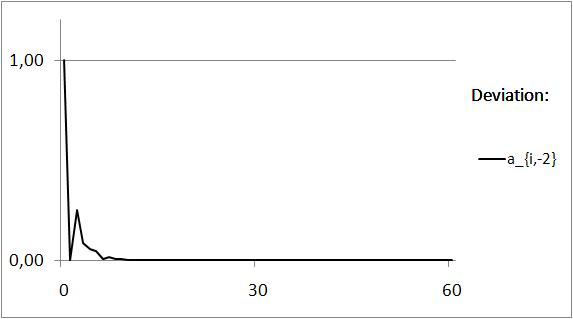
\includegraphics{images/Stieltjes_1_x^3+1.JPG}} 
\end{picture}\\
$$
\rho_1(z) = \rho_2(z) = z^6 + z^3 + 1
$$ \\
\begin{picture}(100,140)(-80,10)
\scalebox{0.5}{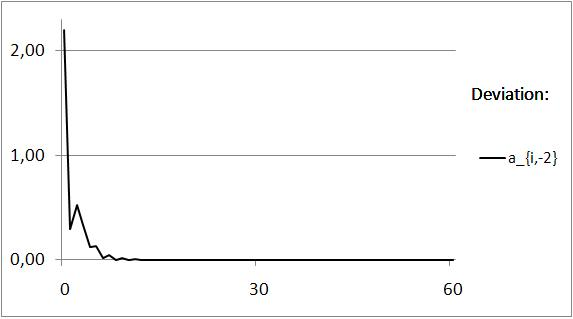
\includegraphics{images/Stieltjes_1_x^6+x^3+1.JPG}} 
\end{picture}\\
$$
\rho_1(z) = z^3 + 1, \rho_2(z) = z^6 + z^3 + 1
$$ \\
\begin{picture}(100,140)(50,10)
\scalebox{0.45}{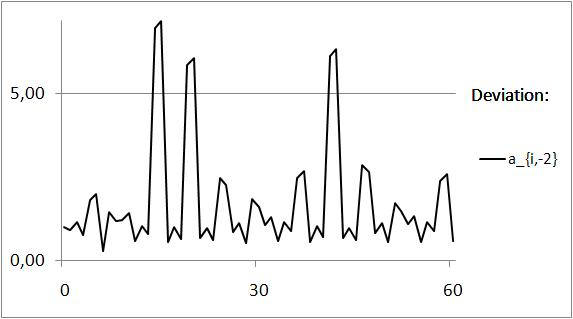
\includegraphics{images/Stieltjes_1_x^3+1_x^6+x^3+1.JPG}} 
\end{picture}
\begin{picture}(100,140)(-120,10)
\scalebox{0.45}{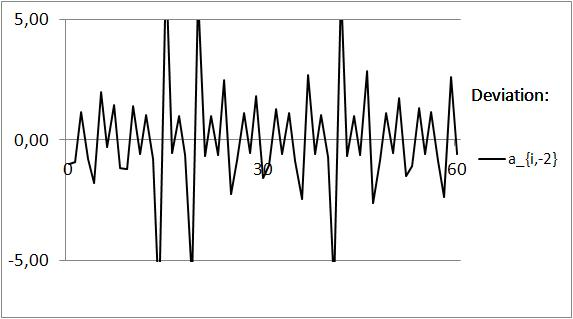
\includegraphics{images/Stieltjes_1_x^3+1_x^6+x^3+1.NOABS.JPG}} 
\end{picture}\\
$$
\rho_1(z) = z^3 + 1, \rho_2(z) = 3z^3 + 3
$$ \\
\begin{picture}(100,140)(-80,10)
\scalebox{0.5}{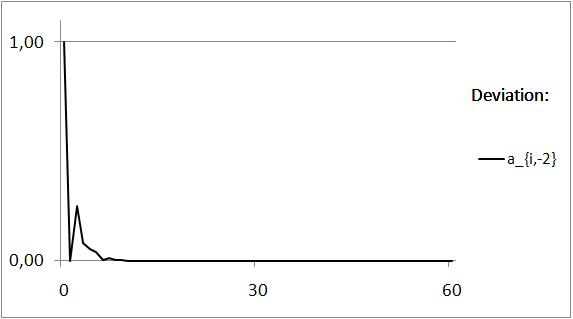
\includegraphics{images/Stieltjes_1_x^3+1_3x^3+3.JPG}} 
\end{picture}\\
$$
\rho_1(z) = z^3 + 1, \rho_2(z) = 3z^3 + 2
$$ \\
\begin{picture}(100,140)(50,10)
\scalebox{0.45}{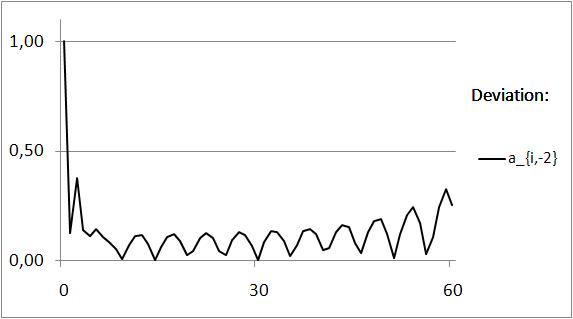
\includegraphics{images/Stieltjes_1_x^3+1_3x^3+2.JPG}} 
\end{picture}
\begin{picture}(100,140)(-120,10)
\scalebox{0.45}{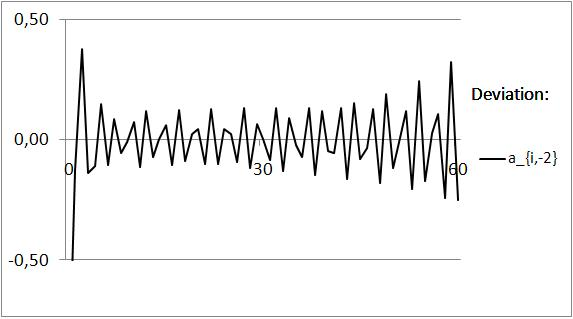
\includegraphics{images/Stieltjes_1_x^3+1_3x^3+2.NOABS.JPG}} 
\end{picture}\\
$$
\rho_1(z) = z^3 + 1, \rho_2(z) = 3z^3 + 1
$$ \\
\begin{picture}(100,140)(50,10)
\scalebox{0.45}{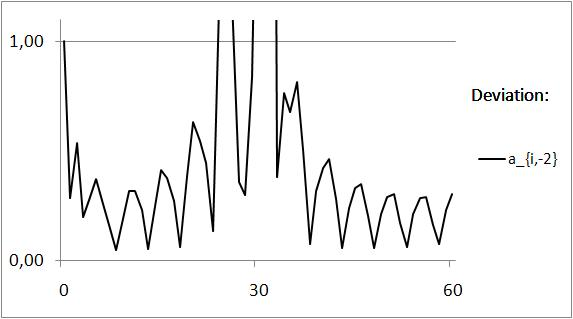
\includegraphics{images/Stieltjes_1_x^3+1_3x^3+1.JPG}} 
\end{picture}
\begin{picture}(100,140)(-120,10)
\scalebox{0.45}{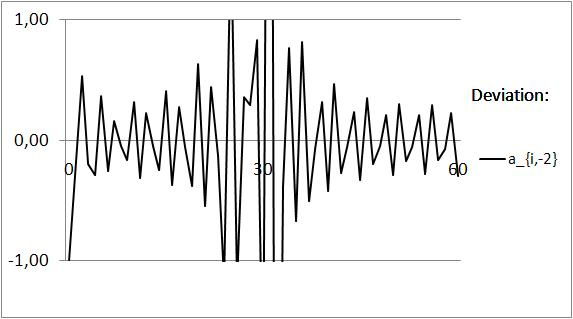
\includegraphics{images/Stieltjes_1_x^3+1_3x^3+1.NOABS.JPG}} 
\end{picture}\\
$$
\rho_1(z) = \rho_2(z) = z^3 - 1
$$ \\
\begin{picture}(100,140)(50,10)
\scalebox{0.45}{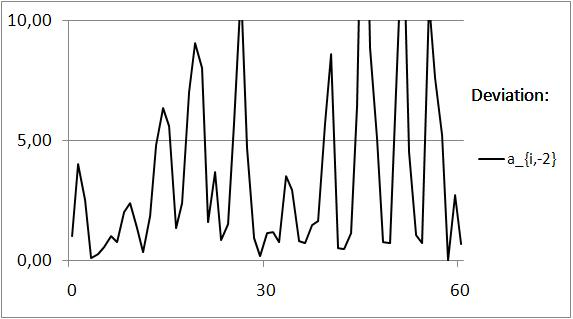
\includegraphics{images/Stieltjes_1_x^3-1.JPG}} 
\end{picture}
\begin{picture}(100,140)(-120,10)
\scalebox{0.45}{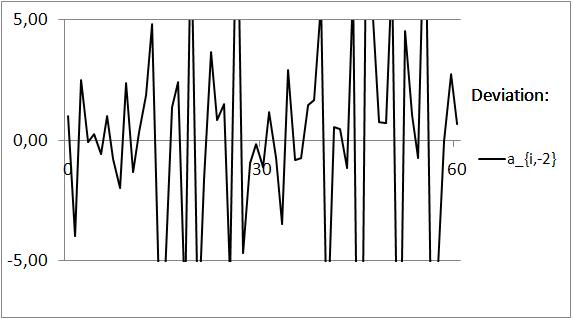
\includegraphics{images/Stieltjes_1_x^3-1.NOABS.JPG}} 
\end{picture}\\

\newpage
\subsection {Системы Никишина}
Пусть $(\sigma_1,\sigma_2,\ldots,\sigma_p)$ некоторые конечные Борелевские меры расположенные на совместно не пересекающихся отрезках 
$\Delta_{j+1} \bigcap \Delta_j =0$ \\
Определим систему мер $(\mu_1, \mu_2,\ldots,\mu_p)$ следующим образом:
$$
 d\mu_1(x) := d\sigma_1 (x),
$$
$$
d\mu_2(x) :=  \langle \sigma_1, \sigma_2 \rangle = \left[ \int_{\Delta_2} \displaystyle\frac{d\sigma_2(z)}{z-x} \right] d\sigma_1(x)
$$
$$
 ...
$$
$$
d\mu_p(x) :=  \langle \sigma_1, \langle \sigma_2, ..., \sigma_p \rangle \rangle, \hspace{0.5cm} x \in \Delta_1 
$$
Система мер $(\mu_1,\mu_2,\ldots,\mu_p)$ называется \it системой Никишина \rm на 
$$\sup \mu_j = \Delta_1, \hspace{0.5cm} j=1,\ldots p$$.
Соответствующие многочлены $Q_n$ для некоторого мульти-индекса $\bf n \rm$ $=(n_1,\ldots,n_p)$ называются \it многочленами Никишина. \rm \\
Для систем Никишина доакзаны следующие важные свойства.
\begin{prope}
Мульти-индексы для $p \leq 3$ строго нормальны, для $p > 3$ это условие пока не доказано.
\end{prope}
\begin{prope}
Реккурентные коэффициенты равномерно ограничены, если носитель $\sigma_1$ компактен.
\end{prope}
\begin{prope}
\label{Nikishin.Limits}
При условии, что $\sigma_k^{'} >0$ везде на носителе $\Delta_k$, тогда для индексов $i \in \{0,\ldots,p-1\}, j \in \{0,\dots,p\}$ существуют следующие пределы $a_{i,-j}^{0}$  реккурентных соотношений
$$
\lim\limits_{k \rightarrow \infty} a_{pk+i, pk+i-j}=a_{i,-j}^{0}
$$
зависящие, только от расположения интервалов носителей.
\end{prope}
Коэффициенты $a_{i,-j}^{0}$ для выбранных носителей при фиксированном $p$ образуют \it референсный оператор. \rm
\begin{prope}
Следствием из (~\ref{Nikishin.Limits}) является то, что любой оператор ассоцированный с некоторой системой Никишина на фиксированных носителях мер при условии, что $\sigma_k^{'} >0$ везде на соответствующем носителе $\Delta_k$ является компактным возмущением референсного оператора. 
\end{prope}

\newpage
\subsection {Системы Никишина $p=2$}
Соответствующие носители для случая $p=2$ определяются как $\Delta_1=[a,0], \Delta_2 =[z_a,1]$, где
$$
z_a=\frac{(a+1)^3}{9(a^2-a+1)} \\
$$
Определим дополнительные переменные:
$$
K:=2a^3-3a^2-3a+2 \\ 
$$
$$
R:=\sqrt{a^2-a+1} \\
$$
Референсный оператор имеет периодическую структуру (период равен 2) 
$$
A_{Nik}^0=
\left(\begin{array}{cccccccccccc}
a_{0,0}  & 1 		& 0 	  & 0 		 &  \cdots \\
a_{1,-1} & a_{1,0}  & 1 	  & 0 		 &  \cdots \\
a_{0,-2} & a_{0,-1} & a_{0,0} & 1 		 &  \cdots \\
0 		 & a_{1,-2} & a_{1,-1} & a_{1,0} &  \cdots \\
\ldots & \ldots & \ldots & \ldots & \ldots
\end{array}\right)
$$
где 
$$
\begin{array}{llllllllllllllll}
a_{0,0} = -\displaystyle\frac {1}{36R^2} [K - 12(a+1)R^2+10R^3] & a_{1,0}=-\displaystyle\frac{1}{18R^2}[K-6(a+1)R^2+4R^3] \\ \\ 
a_{0,-1}= -\displaystyle\frac {1}{36^2R^4}(-K+2R^3)(K-14R^3) & a_{1,-1}=-\displaystyle\frac{1}{36^2R^4}(-K+2R^3)(K-14R^3) \\ \\
a_{0,-2}= -\displaystyle\frac {1}{36 \cdot 81 R^3}(-K+2R^3)^2 & a_{1,-2}=-\displaystyle\frac{1}{36^3R^6}(-K+2R^3)^2(K+2R^3) \\
\end{array}
$$
Обозначим через $\mu_1^0, \mu_2^0$ меры соответствующие референсному оператору.
В следующих главах мы рассмотрим различные полиномиальные возмущения исходных мер весовыми функциями
$$
d\mu_1(z)= \rho_1(z) d\mu_1^0 (z) , \hspace{0.5cm} d\mu_2(z) =  \rho_2(z) \mu^0_2(z)
$$
Проверим на практике условия компактности возмущения оператора. 
Для каждого примера левый график показывает полином, правый график показывает отклонения (по модулю) получающихся реккурентных соотношений от референсного оператора $A_{Nik}^0$  


\newpage
\subsection {Система Никишина $\Delta_1=[-1,0], \Delta_2 =[0,1]$}
Рассмотрим случай $a=-1$
$$
z_a = 0, K = 0, R = \sqrt{3}
$$
Референсный оператор
$$
A_{Nik}^0=
\left(\begin{array}{cccccccccccc}
-\displaystyle\frac{5}{4}\alpha & 1 & 0 & 0 &  \cdots \\
\displaystyle\frac{7}{16}\alpha^2 & -\alpha & 1 & 0 &  \cdots \\
-\displaystyle\frac{1}{8}\alpha^3 & \displaystyle\frac{7}{16}\alpha^2 & -\displaystyle\frac{5}{4}\alpha & 1 &  \cdots \\
0 & -\displaystyle\frac{1}{64}\alpha^3 & \displaystyle\frac{7}{16}\alpha^2 & -\alpha &  \cdots \\
\ldots & \ldots & \ldots & \ldots & \ldots
\end{array}\right)
$$
где $\alpha=2/(3\sqrt{3})$ \\
$$
\rho_1(z) = \rho_2(z) = \displaystyle\left(\frac{1}{2}+z \right)^2
$$
\begin{picture}(100,140)(10,10)
\scalebox{0.5}{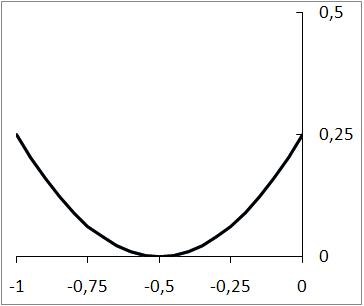
\includegraphics{images/(1_2+x)^2_-1_0.JPG}} 
\end{picture}
\begin{picture}(100,140)(-80,10)
\scalebox{0.5}{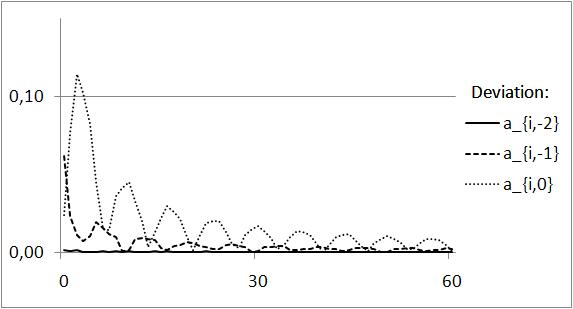
\includegraphics{images/(1_2+x)^2_Nikishin.JPG}} 
\end{picture}\\
$$
\rho_1(z) = \rho_2(z) = z^3+1
$$
\begin{picture}(100,140)(10,10)
\scalebox{0.5}{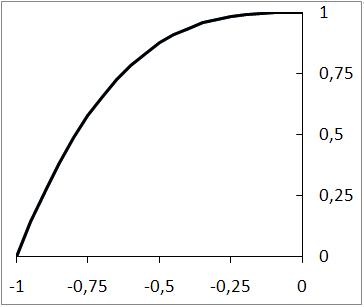
\includegraphics{images/x^3+1_-1_0.JPG}} 
\end{picture}
\begin{picture}(100,140)(-80,10)
\scalebox{0.5}{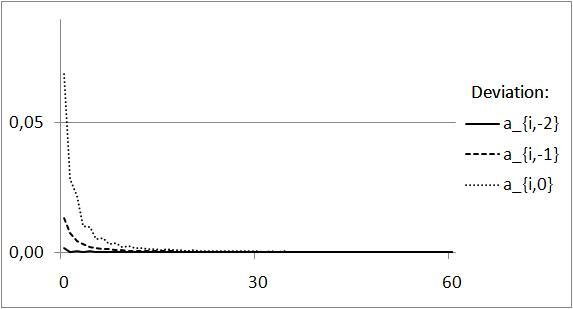
\includegraphics{images/x^3+1_Nikishin.JPG}} 
\end{picture}\\ \\
$$
\rho_1(z) = \rho_2(z) = -z
$$
\begin{picture}(100,140)(10,10)
\scalebox{0.5}{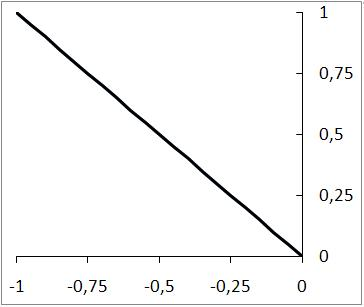
\includegraphics{images/-x_-1_0.JPG}} 
\end{picture}
\begin{picture}(100,140)(-80,10)
\scalebox{0.5}{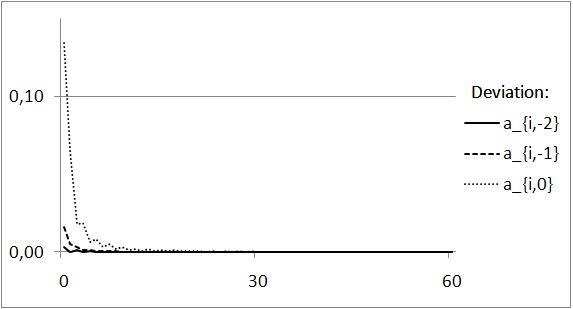
\includegraphics{images/-z_Nikishin.JPG}} 
\end{picture}\\
$$
\rho_1(z) = \rho_2(z) = z^3-z
$$
\begin{picture}(100,140)(10,10)
\scalebox{0.5}{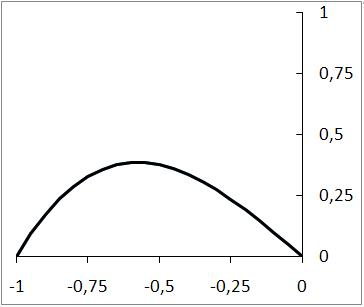
\includegraphics{images/x^3-x_-1_0.JPG}} 
\end{picture}
\begin{picture}(100,140)(-80,10)
\scalebox{0.5}{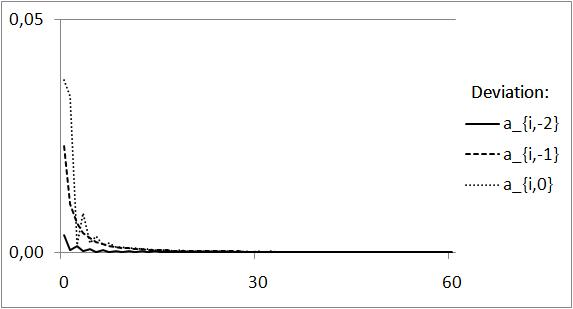
\includegraphics{images/x^3-x_Nikishin.JPG}} 
\end{picture}\\ \\
$$
\rho_1(z) = -z, \rho_2(z) = z + 1
$$
\begin{picture}(100,140)(10,10)
\scalebox{0.5}{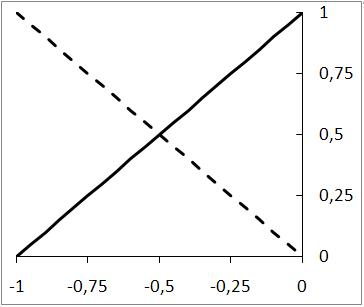
\includegraphics{images/-x_x+1_-1_0.JPG}} 
\end{picture}
\begin{picture}(100,140)(-80,10)
\scalebox{0.5}{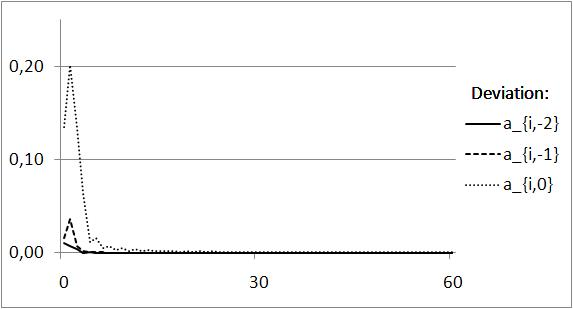
\includegraphics{images/-x_x+1_Nikishin.JPG}} 
\end{picture}\\
$$
\rho_1(z) = -z, \rho_2(z) = z^3 + 1
$$
\begin{picture}(100,140)(10,10)
\scalebox{0.5}{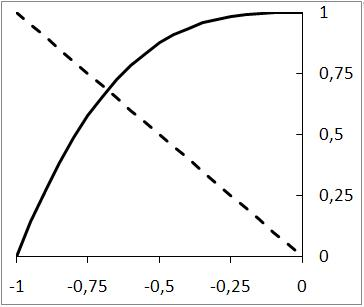
\includegraphics{images/-x_x^3+1_-1_0.JPG}} 
\end{picture}
\begin{picture}(100,140)(-80,10)
\scalebox{0.5}{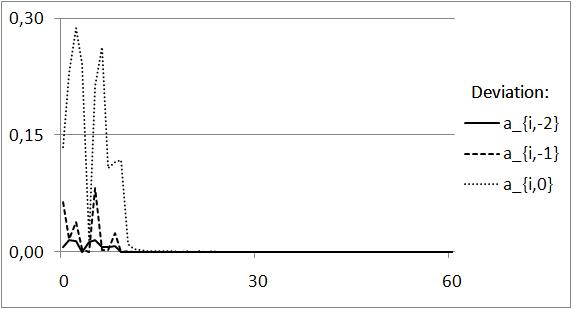
\includegraphics{images/-x_x^3+1_Nikishin.JPG}} 
\end{picture}\\ \\ \\
\begin{picture}(100,140)(-80,10)
\scalebox{0.5}{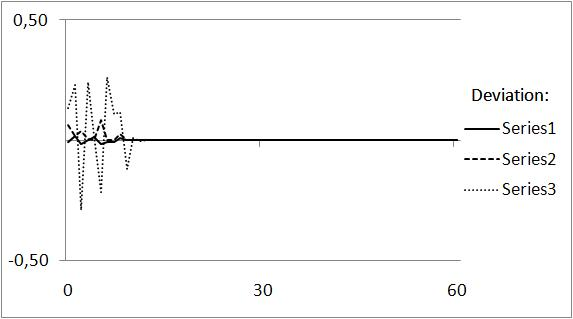
\includegraphics{images/-x_x^3+1_Nikishin.NOABS.JPG}} 
\end{picture} \\ \\
$$
\rho_1(z) = \rho_2(z) = \displaystyle\frac{1}{2}+z
$$
\begin{picture}(100,140)(10,10)
\scalebox{0.5}{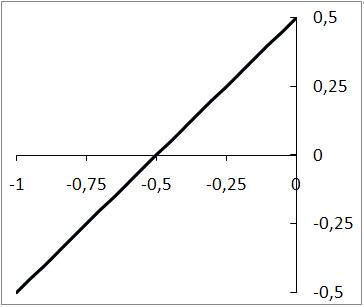
\includegraphics{images/1_2+x_-1_0.JPG}} 
\end{picture}
\begin{picture}(100,140)(-80,10)
\scalebox{0.5}{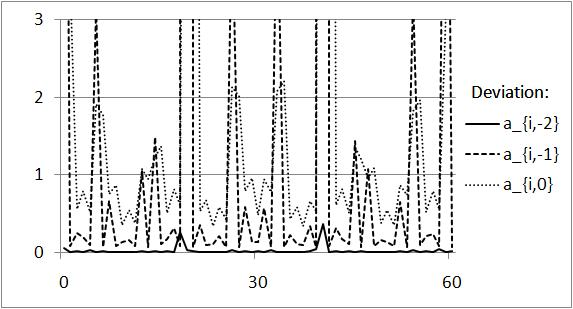
\includegraphics{images/1_2+x_Nikishin.JPG}} 
\end{picture}\\ \\ \\
\begin{picture}(100,140)(-80,10)
\scalebox{0.5}{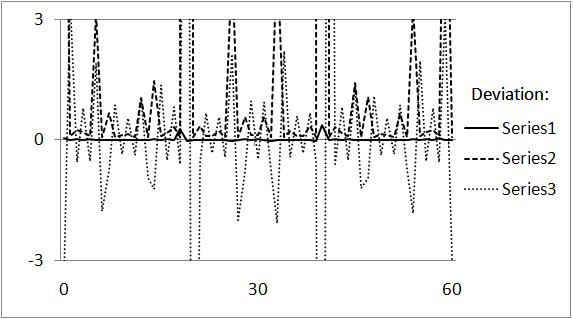
\includegraphics{images/1_2+x_Nikishin.NOABS.JPG}} 
\end{picture}

\newpage
\subsection {Система Никишина $\Delta_1=[-1/2,0], \Delta_2 =[z_a,1]$}
При $a=-1/2$
$$
z_a = \displaystyle\frac{1}{126}, K = \displaystyle{5}{2}, R = \displaystyle\frac{\sqrt{7}}{2}
$$
Референсный оператор 
$$
\begin{array}{llllllllllllllll}
a_{0,0} = \displaystyle\frac {8}{63}-\displaystyle\frac{5}{36}\sqrt{7} & a_{1,0}=\displaystyle\frac{11}{126}-\displaystyle\frac{1}{9}\sqrt{7} \\ \\ 
a_{0,-1}= a_{1,-1}= \displaystyle\frac{2501}{63504}-\displaystyle\frac{5}{567}\sqrt{7} \\ \\
a_{0,-2}= \displaystyle\frac {-443}{285768}\sqrt{7}+ \displaystyle\frac {5}{1458} & a_{1,-2}= \displaystyle\frac {5}{32928}- \displaystyle\frac {1}{9408}\sqrt{7}\\
\end{array}
$$
Рассмотрим различные полиномиальные возмущения \\
$$
\rho_1(z) = \rho_2(z) = \displaystyle\left(\frac{1}{2}+z \right)^2
$$
\begin{picture}(100,140)(10,10)
\scalebox{0.5}{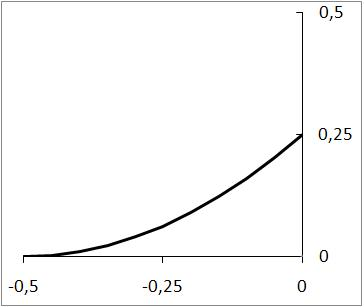
\includegraphics{images/(1_2+x)^2_-1_2_0.JPG}} 
\end{picture}
\begin{picture}(100,140)(-80,10)
\scalebox{0.5}{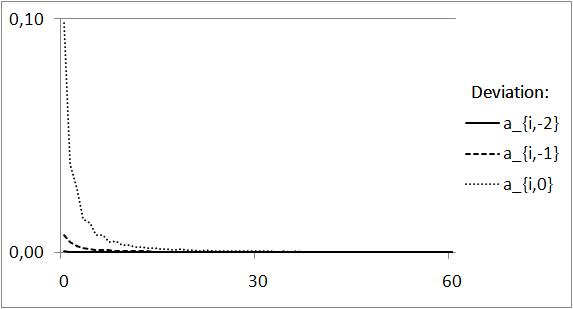
\includegraphics{images/Nikishin_-05_(1_2+x)^2.JPG}} 
\end{picture}\\ 
$$
\rho_1(z) = \rho_2(z) = z^3+1
$$
\begin{picture}(100,140)(10,10)
\scalebox{0.5}{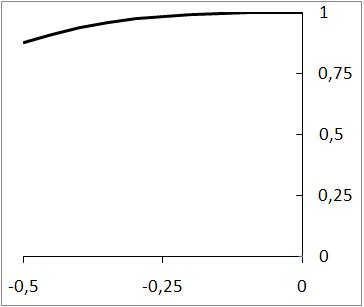
\includegraphics{images/x^3+1_-1_2_0.JPG}} 
\end{picture}
\begin{picture}(100,140)(-80,10)
\scalebox{0.5}{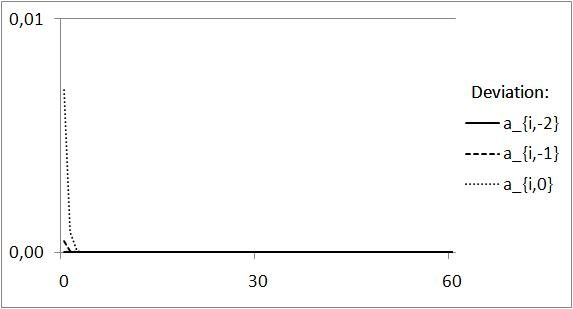
\includegraphics{images/Nikishin_-05_x^3+1.JPG}} 
\end{picture}\\ 
$$
\rho_1(z) = \rho_2(z) = -z
$$
\begin{picture}(100,140)(10,10)
\scalebox{0.5}{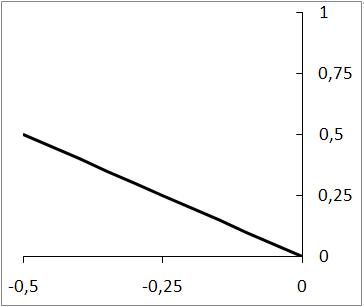
\includegraphics{images/-x_-1_2_0.JPG}} 
\end{picture}
\begin{picture}(100,140)(-80,10)
\scalebox{0.5}{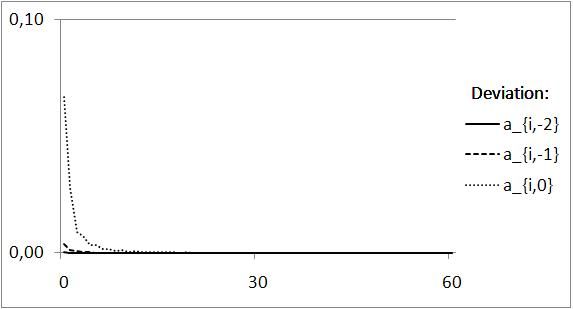
\includegraphics{images/Nikishin_-05_-x.JPG}} 
\end{picture}\\ 
$$
\rho_1(z) = \rho_2(z) = z^3-z
$$
\begin{picture}(100,140)(10,10)
\scalebox{0.5}{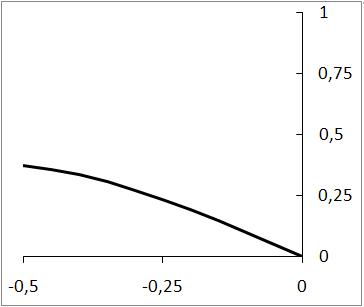
\includegraphics{images/x^3-x_-1_2_0.JPG}} 
\end{picture}
\begin{picture}(100,140)(-80,10)
\scalebox{0.5}{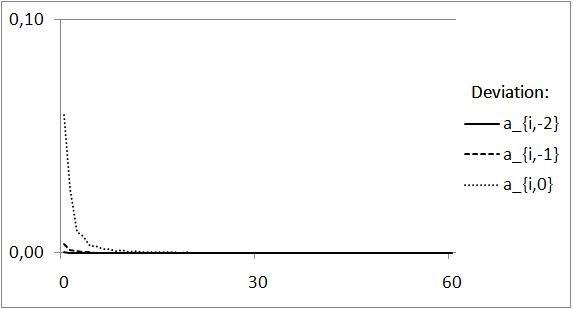
\includegraphics{images/Nikishin_-05_x^3-x.JPG}} 
\end{picture}\\ 
$$
\rho_1(z) = -z, \rho_2(z) = z+1
$$
\begin{picture}(100,140)(10,10)
\scalebox{0.5}{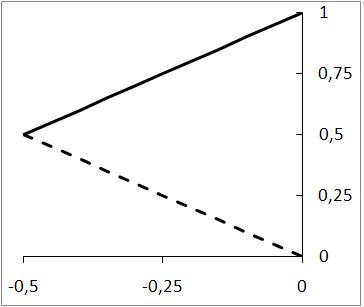
\includegraphics{images/-x_x+1_-1_2_0.JPG}} 
\end{picture}
\begin{picture}(100,140)(-80,10)
\scalebox{0.5}{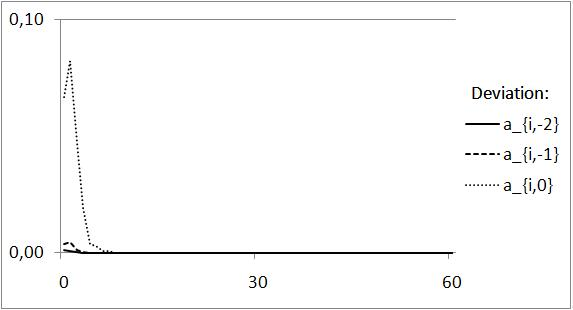
\includegraphics{images/Nikishin_-05_-x_x+1.JPG}} 
\end{picture}\\ 
$$
\rho_1(z) = -z, \rho_2(z) = z^3+1
$$
\begin{picture}(100,140)(10,10)
\scalebox{0.5}{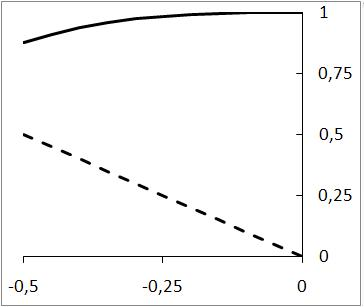
\includegraphics{images/-x_x^3+1_-1_2_0.JPG}} 
\end{picture}
\begin{picture}(100,140)(-80,10)
\scalebox{0.5}{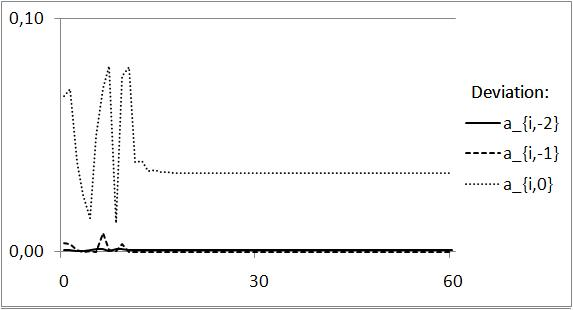
\includegraphics{images/Nikishin_-05_-x_x^3+1.JPG}} 
\end{picture}\\ \\
$$
\rho_1(z) = \rho_2(z) = \displaystyle\frac{1}{2}+z
$$
\begin{picture}(100,140)(10,10)
\scalebox{0.5}{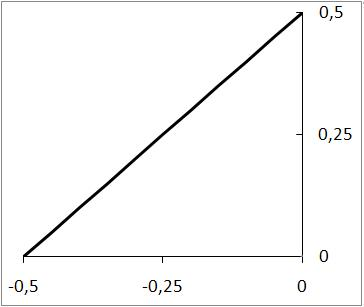
\includegraphics{images/1_2+x_-1_2_0.JPG}} 
\end{picture}
\begin{picture}(100,140)(-80,10)
\scalebox{0.5}{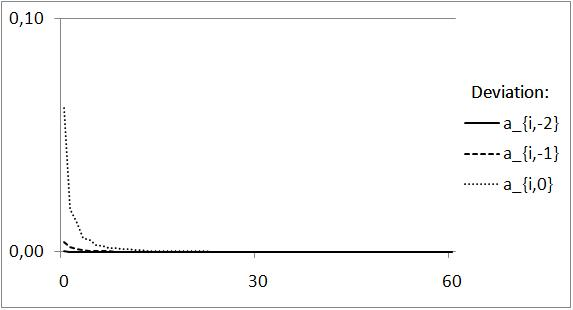
\includegraphics{images/Nikishin_-05_05+x.JPG}} 
\end{picture}\\ 
$$
\rho_1(z) = \rho_2(z) = \displaystyle\frac{1}{4}+z
$$
\begin{picture}(100,140)(10,10)
\scalebox{0.5}{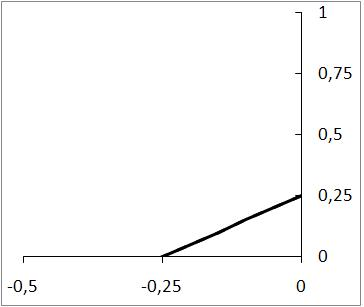
\includegraphics{images/1_4+x_-1_2_0.JPG}} 
\end{picture}
\begin{picture}(100,140)(-80,10)
\scalebox{0.5}{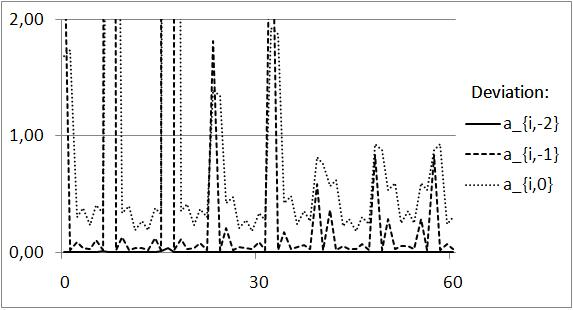
\includegraphics{images/Nikishin_-05_025+x.JPG}} 
\end{picture}\\ 
$$
\rho_1(z) = \displaystyle\frac{1}{2}-z, \rho_2(z) = 1-z
$$
\begin{picture}(100,140)(10,10)
\scalebox{0.5}{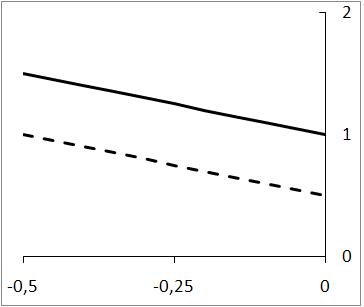
\includegraphics{images/1_2-x_1-x_-1_2_0.JPG}} 
\end{picture}
\begin{picture}(100,140)(-80,10)
\scalebox{0.5}{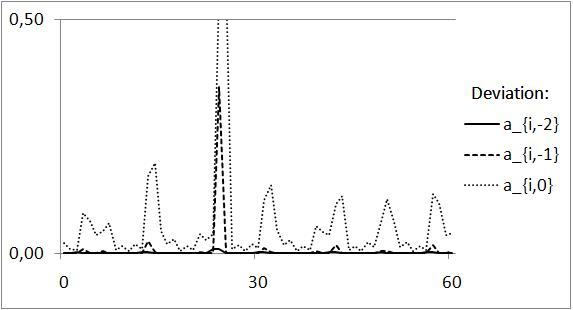
\includegraphics{images/Nikishin_-05_05-x_1-x.JPG}} 
\end{picture}\\ 
$$
\rho_1(z) = z^2+2, \rho_2(z) = 2-z^3
$$
\begin{picture}(100,140)(10,10)
\scalebox{0.5}{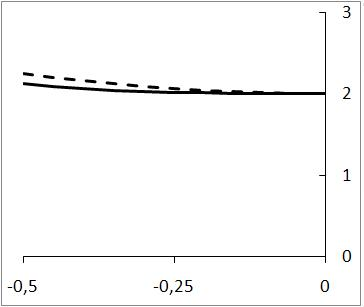
\includegraphics{images/x^2+2_2-x^3_-1_2_0.JPG}} 
\end{picture}
\begin{picture}(100,140)(-80,10)
\scalebox{0.5}{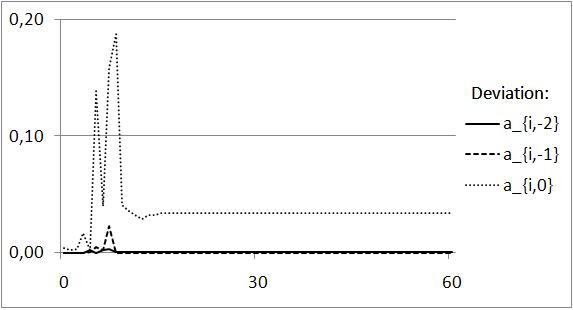
\includegraphics{images/Nikishin_-05_x^2+2_2-x^3.JPG}} 
\end{picture}\\ 
$$
\rho_1(z) = -z, \rho_2(z) = z
$$
\begin{picture}(100,140)(10,10)
\scalebox{0.5}{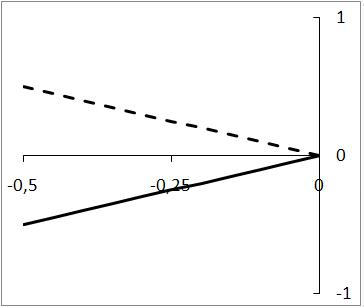
\includegraphics{images/-x_x_-1_2_0.JPG}} 
\end{picture}
\begin{picture}(100,140)(-80,10)
\scalebox{0.5}{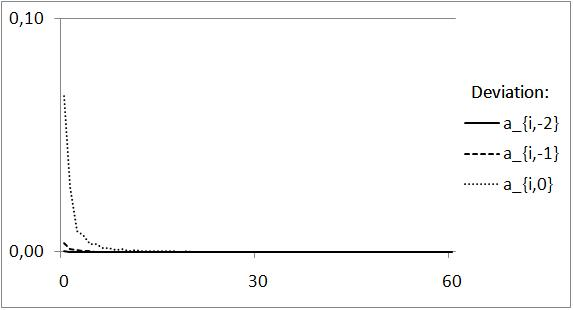
\includegraphics{images/Nikishin_-05_-x_x.JPG}} 
\end{picture}\\ \\

\newpage
\subsection {Система Никишина $\Delta_1=[-3/4,0], \Delta_2 =[z_a,1]$}
При $a=-3/4$
$$
z_a = \displaystyle\frac{1}{1332}, K = \displaystyle{55}{32}, R = \displaystyle\frac{\sqrt{37}}{4}
$$
Коэффициенты референсного оператора: 
$$
\begin{array}{llllllllllllllll}
a_{0,0} = \displaystyle\frac {167}{2664}-\displaystyle\frac{5}{72}\sqrt{37} & a_{1,0}=\displaystyle\frac{14}{333}-\displaystyle\frac{1}{18}\sqrt{37} \\ \\ 
a_{0,-1}= a_{1,-1}= \displaystyle\frac{89399}{1774224}-\displaystyle\frac{55}{23976}\sqrt{37} \\ \\
a_{0,-2}= \displaystyle\frac {-26839}{31936032}\sqrt{37}+ \displaystyle\frac {55}{23328} & a_{1,-2}= \displaystyle\frac {2695}{19450752}- \displaystyle\frac {49}{525696}\sqrt{37}\\
\end{array}
$$
Рассмотрим различные полиномиальные возмущения 
$$
\rho_1(z) = \rho_2(z) = \displaystyle\left(\frac{1}{2}+z \right)^2
$$
\begin{picture}(100,140)(10,10)
\scalebox{0.5}{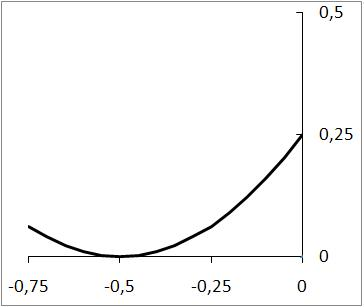
\includegraphics{images/(1_2+x)^2_-3_4_0.JPG}} 
\end{picture}
\begin{picture}(100,140)(-80,10)
\scalebox{0.5}{\includegraphics{images/Nikishin_-0.75_(1_2+x)^2.JPG}} 
\end{picture}\\ 
$$
\rho_1(z) = \rho_2(z) = z^3+1
$$
\begin{picture}(100,140)(10,10)
\scalebox{0.5}{\includegraphics{images/x^3+1_-3_4_0.JPG}} 
\end{picture}
\begin{picture}(100,140)(-80,10)
\scalebox{0.5}{\includegraphics{images/Nikishin_-0.75_x^3+1.JPG}} 
\end{picture}\\ 
$$
\rho_1(z) = \rho_2(z) = -z
$$
\begin{picture}(100,140)(10,10)
\scalebox{0.5}{\includegraphics{images/-x_-3_4_0.JPG}} 
\end{picture}
\begin{picture}(100,140)(-80,10)
\scalebox{0.5}{\includegraphics{images/Nikishin_-0.75_-x.JPG}} 
\end{picture}\\ 
$$
\rho_1(z) = \rho_2(z) = z^3-z
$$
\begin{picture}(100,140)(10,10)
\scalebox{0.5}{\includegraphics{images/x^3-x_-3_4_0.JPG}} 
\end{picture}
\begin{picture}(100,140)(-80,10)
\scalebox{0.5}{\includegraphics{images/Nikishin_-0.75_x^3-x.JPG}} 
\end{picture}\\ 
$$
\rho_1(z) = -z, \rho_2(z) = z+1
$$
\begin{picture}(100,140)(10,10)
\scalebox{0.5}{\includegraphics{images/-x_x+1_-3_4_0.JPG}} 
\end{picture}
\begin{picture}(100,140)(-80,10)
\scalebox{0.5}{\includegraphics{images/Nikishin_-0.75_-x_x+1.JPG}} 
\end{picture}\\ 
$$
\rho_1(z) = -z, \rho_2(z) = z^3+1
$$
\begin{picture}(100,140)(10,10)
\scalebox{0.5}{\includegraphics{images/-x_x^3+1_-3_4_0.JPG}} 
\end{picture}
\begin{picture}(100,140)(-80,10)
\scalebox{0.5}{\includegraphics{images/Nikishin_-0.75_-x_x^3+1.JPG}} 
\end{picture}\\ 
$$
\rho_1(z) = \rho_2(z) = \displaystyle\frac{1}{2}+z
$$
\begin{picture}(100,140)(10,10)
\scalebox{0.5}{\includegraphics{images/1_2+x_-3_4_0.JPG}} 
\end{picture}
\begin{picture}(100,140)(-80,10)
\scalebox{0.5}{\includegraphics{images/Nikishin_-0.75_0.5+x.JPG}} 
\end{picture}\\ 
$$
\rho_1(z) = \rho_2(z) = \displaystyle\frac{3}{4}+z
$$
\begin{picture}(100,140)(10,10)
\scalebox{0.5}{\includegraphics{images/3_4+x_-3_4_0.JPG}} 
\end{picture}
\begin{picture}(100,140)(-80,10)
\scalebox{0.5}{\includegraphics{images/Nikishin_-0.75_0.75+x.JPG}} 
\end{picture}\\ 
$$
\rho_1(z) = \displaystyle\frac{1}{2}-z, \rho_2(z) = 1-z
$$
\begin{picture}(100,140)(10,10)
\scalebox{0.5}{\includegraphics{images/1_2-x_1-x_-3_4_0.JPG}} 
\end{picture}
\begin{picture}(100,140)(-80,10)
\scalebox{0.5}{\includegraphics{images/Nikishin_-0.75_0.5-x_1-x.JPG}} 
\end{picture}\\ 
$$
\rho_1(z) = z^2+2, \rho_2(z) = 2-z^3
$$
\begin{picture}(100,140)(10,10)
\scalebox{0.5}{\includegraphics{images/x^2+2_2-x^3_-3_4_0.JPG}} 
\end{picture}
\begin{picture}(100,140)(-80,10)
\scalebox{0.5}{\includegraphics{images/Nikishin_-0.75_x^2+2_2-x^3.JPG}} 
\end{picture}\\ 
$$
\rho_1(z) = -z, \rho_2(z) = z
$$
\begin{picture}(100,140)(10,10)
\scalebox{0.5}{\includegraphics{images/-x_x_-3_4_0.JPG}} 
\end{picture}
\begin{picture}(100,140)(-80,10)
\scalebox{0.5}{\includegraphics{images/Nikishin_-0.75_-x_x.JPG}} 
\end{picture}\\ \\







\newpage
\subsection {Системы Анжелеско}
Система борелевских мер $\mu_1,\ldots \mu_p$ таких, что носители мер не имеют
общих внутренних точек ${\Delta_i}\cap{\Delta_j} = 0, i\not=j $ называется \it системой Анжелеско \rm. \\
Для систем Анжелеско доказано несколько важных свойств.
\begin{prope}
Все мульти-индексы $\bf n \rm$ $=(n_1,\ldots,n_p)$ строго нормальны.
\end{prope}
\begin{prope}
Соответствующий разностный оператор ограничен, если носители мер $\Delta_1, \ldots \Delta_p$ компактны.
\end{prope}
\begin{prope}
\label{Angelesco.limits}
Если меры $\mu_1, \ldots \mu_p$ удовлетворяют условию Сег\"{е}, 
$$
d\mu_j(x)=\rho(x)dx
$$
$$
\int_{\Delta_j} \log \rho_j(x) dx > - \infty, \hspace{0.5cm} j=1,\ldots p
$$
тогда существуют пределы реккурентных коэффициентов с периодичностью $p$  
\end{prope}
\begin{prope}
Следствием из (~\ref{Angelesco.limits}) является то, что любой оператор чьи резольвентные функции образуют систему Анжелеско меры которой удовлетворяют условию Сег\"{е} является компактным возмущением референсного оператора, коэффициенты которого в свою очередь имеют пределы с периодом $p$ 
\end{prope}



\newpage
\subsection {Системы Чебышева $p=2$ на $\Delta_1=[-1,0], \Delta_2 =[0,1]$}
Рассмотрим меру $$\rho_1(z)=\displaystyle\frac{1}{\sqrt{1-x^2}}$$ на носителе  $[-1,0]$ и меру $$\rho_2(z)=\sqrt{1-x^2}$$ на носителе $[0,1]$ \\
Меры соответствуют классическим ортогональным многочленма Чебышева 1-го $T_n(z)$ и 2-го $U_n(z)$ рода соответственно
$$
T_0 = 1, T_1=z, \ldots T_{n+1}(z)=2zT_n(z)-T_{n-1}(z)
$$
$$
U_0 = 1, U_1=2z, \ldots U_{n+1}(z)=2zT_n(z)-T_{n-1}(z)
$$

\subsubsection {Модифицированный алгоритм Чебышева. Полиномиальные возмущения.}
Рассмотрим различные полиномиальные возмущения
$$
\rho_1(z) = \rho_2(z) = \displaystyle\left(\frac{1}{2}+z \right)^2
$$ \\
\begin{picture}(100,140)(10,10)
\scalebox{0.5}{\includegraphics{images/(1_2+x)^2.JPG}} 
\end{picture}
\begin{picture}(100,140)(-80,10)
\scalebox{0.5}{\includegraphics{images/(1_2+x)^2_Chebushev.JPG}} 
\end{picture}\\
$$
\rho_1(z) = \rho_2(z) = z^3+1
$$ \\
\begin{picture}(100,140)(10,10)
\scalebox{0.5}{\includegraphics{images/x^3+1.JPG}} 
\end{picture}
\begin{picture}(100,140)(-80,10)
\scalebox{0.5}{\includegraphics{images/x^3+1_Chebushev.JPG}} 
\end{picture}\\ \\
$$
\rho_1(z) = \rho_2(z) = -z
$$ \\
\begin{picture}(100,140)(10,10)
\scalebox{0.5}{\includegraphics{images/-z.JPG}} 
\end{picture}
\begin{picture}(100,140)(-80,10)
\scalebox{0.5}{\includegraphics{images/-z_Chebushev.JPG}} 
\end{picture}\\
$$
\rho_1(z) = \rho_2(z) = z^3-z
$$ \\
\begin{picture}(100,140)(10,10)
\scalebox{0.5}{\includegraphics{images/x^3-x.JPG}} 
\end{picture}
\begin{picture}(100,140)(-80,10)
\scalebox{0.5}{\includegraphics{images/x^3-x_Chebushev.JPG}} 
\end{picture}\\ \\
$$
\rho_1(z) = -z, \rho_2(z) = z + 1
$$ \\
\begin{picture}(100,140)(10,10)
\scalebox{0.5}{\includegraphics{images/-x_x+1.JPG}} 
\end{picture}
\begin{picture}(100,140)(-80,10)
\scalebox{0.5}{\includegraphics{images/-x_x+1_Chebushev.JPG}} 
\end{picture}\\ \\ \\ \\
\begin{picture}(100,140)(-80,10)
\scalebox{0.5}{\includegraphics{images/-x_x+1_Chebushev.NOABS.JPG}} 
\end{picture} \\ \\
$$
\rho_1(z) = z^2-3z+2, \rho_2(z) = z^2 + 3z + 2
$$ \\
\begin{picture}(100,140)(10,10)
\scalebox{0.5}{\includegraphics{images/x^2-3x+2_x^2+3x+2.JPG}} 
\end{picture}
\begin{picture}(100,140)(-80,10)
\scalebox{0.5}{\includegraphics{images/x^2-3x+2_x^2+3x+2_Chebushev.JPG}} 
\end{picture}\\
 \\
$$
\rho_1(z) = \rho_2(z) = \displaystyle\frac{1}{2}+z
$$ \\
\begin{picture}(100,140)(10,10)
\scalebox{0.5}{\includegraphics{images/1_2+x.JPG}} 
\end{picture}
\begin{picture}(100,140)(-80,10)
\scalebox{0.5}{\includegraphics{images/1_2+x_Chebushev.JPG}} 
\end{picture}\\ \\ \\ \\
\begin{picture}(100,140)(-80,10)
\scalebox{0.5}{\includegraphics{images/1_2+x_Chebushev.NOABS.JPG}} 
\end{picture} \\ \\
$$
\rho_1(z) = -z, \rho_2(z) = -z + 1
$$ \\
\begin{picture}(100,140)(10,10)
\scalebox{0.5}{\includegraphics{images/-x_-x+1.JPG}} 
\end{picture}
\begin{picture}(100,140)(-80,10)
\scalebox{0.5}{\includegraphics{images/-x_-x+1_Chebushev.JPG}} 
\end{picture}\\ \\ \\ \\
\begin{picture}(100,140)(-80,10)
\scalebox{0.5}{\includegraphics{images/-x_-x+1_Chebushev.NOABS.JPG}} 
\end{picture} \\ \\
$$
\rho_1(z) = z^2+2, \rho_2(z) = 2-x^3
$$ \\
\begin{picture}(100,140)(10,10)
\scalebox{0.5}{\includegraphics{images/x^2+2_2-x^3.JPG}} 
\end{picture}
\begin{picture}(100,140)(-80,10)
\scalebox{0.5}{\includegraphics{images/x^2+2_2-x^3_Chebushev.JPG}} 
\end{picture}\\ \\

\chapter {Обратная спектральная задача. Процедура Стильтеса.}
В качестве одного из решений
обратной спектральной задачи рассмотрим процедуру
Стилтъеса. \\
Основная идея процедуры Стилтъеса - вычисление коэффициентов $a_{i,j}$ рекуррентного соотношения напрямую через вычисление функционалов $L_j(Q_i,Q_k)$. \\
Функционалы в свою очередь вычисляются через квадратуру Гаусса.
\begin{equation}
L_j(Q_i,Q_k)=\sum\limits_{t=0}^{n-1}{Q_i(\lambda_{t})Q_k(\lambda_{t})r_{t}^{(j)}}
\end{equation}
где $n$ количество узлов квадратуры, $\lambda_t$ - узлы и $r_{t}$
- веса квадратуры.\\
Процедура стартует со следующих начальные условий:
$$Q_0=1, a_{0,0}=\frac{\displaystyle{L_1(Q_0,zQ_0)}}{\displaystyle{L_1(O_0,Q_0)}}$$ \\
Далее последовательно для $i=1,\ldots,n-1$ \\
1. Вычислить многочлен $Q_i$ из реккурентного соотношения (~\ref{StieltO}), пользуясь вычисленными многочленами и коэффициентами с предыдущего шага: 
$$Q_{i-1}, \ldots, Q_{i-1-p}; \mbox{    } a_{i-1,i-1-p}, \ldots,a_{i-1, i-1-p}$$  \\ 
2. Вычислить поcледовательно коэффициенты 
$$a_{i,i-p}, \ldots, a_{i,i}$$ используя выражения (~\ref{StieltA}).\\
\newpage
\subsection {Система Чебышева $p=2, \Delta_1=[-1,0], \Delta_2=[0,1]$. Возмущения точками масс.}
Рассмотрим различные возмущения различными массами на примере 
системы Чебышева 1-го рода $$\rho_1(z)=\displaystyle\frac{1}{\sqrt{1-x^2}}$$ на носителе $[-1,0]$ и системы Чебышева 2-го рода $$\rho_2(z)=\sqrt{1-x^2}$$ на носителе $[0,1]$ \\

\subsubsection {Квадратура Чебышева}
Для системы Чебышева 1-го рода известна следующая квадратура.
Для некоторого интервала $[a,b]$ и целого $n$ узлы квадратуры выражаются: 
$$\lambda_i = \frac{a+b}{2} + \frac{b-a}{2}cos\left(\frac{ (2i-1)\pi}{2n}\right),i=1,\ldots,n$$
Веса квадратуры
$$\tau_i=\frac{1}{n},i=1,\ldots,n$$
Для системы Чебышева 2-го рода известна следующая квадратура.
Для некоторого интервала $[a,b]$ и целого $n$ узлы квадратуры выражаются: 
$$\lambda_i =\frac{a+b}{2} + \frac{b-a}{2}cos\left(\frac{i \pi}{n+1}\right), i=1,\ldots,n$$
Веса квадратуры
$$\tau_i=\frac{2}{n+1} sin^2 \left( \frac{i \pi}{n+1} \right),i=1,\ldots,n$$ \\
\\
$$
[-2;0.5] [2;0.5]
$$ \\
\begin{picture}(100,140)(10,10)
\scalebox{0.5}{\includegraphics{images/-2_2.JPG}} 
\end{picture}
\begin{picture}(100,140)(-80,10)
\scalebox{0.5}{\includegraphics{images/-2_2_128.JPG}} 
\end{picture}\\ \\
$$
[-2;0.5] [-0.9;0.1] [0.9;0.1] [1;0.2]
$$ \\
\begin{picture}(100,140)(10,10)
\scalebox{0.5}{\includegraphics{images/-2_-0,9_0,9_1.JPG}} 
\end{picture}
\begin{picture}(100,140)(-80,10)
\scalebox{0.5}{\includegraphics{images/-2_-0,9_0,9_1_128.JPG}} 
\end{picture}\\ \\
$$
[-2;0.2] [-0.9;0.1] [-0.1;0.1] [0.1;0.1] [0.9;0.1] [2;0.2]
$$ \\
\begin{picture}(100,140)(10,10)
\scalebox{0.5}{\includegraphics{images/-2_-0,9_-0,1_0,1_0,9_2.JPG}} 
\end{picture}
\begin{picture}(100,140)(-80,10)
\scalebox{0.5}{\includegraphics{images/-2_-0,9_-0,1_0,1_0,9_2_128.JPG}} 
\end{picture}\\ \\
$$
[-1,0.1] [3;0.5]
$$ \\
\begin{picture}(100,140)(10,10)
\scalebox{0.5}{\includegraphics{images/-1_3.JPG}} 
\end{picture}
\begin{picture}(100,140)(-80,10)
\scalebox{0.5}{\includegraphics{images/-1_3_128.JPG}} 
\end{picture}\\ \\

\subsubsection {Система Чебышева $p=2, \Delta_1=[-1,-0.5], \Delta_2=[0.5,1]$. Возмущения точками масс.}


\subsection{Процедура Стильтеса для $\Delta_1=[-a,0], \Delta_2=[0,1]$}
Рассмотрим результаты процедуры Стильтеса для различных участков носителей мер Чебышева 1-го и 2-го рода с одной общей точкой - ноль, $a=1, 0.75, 0.5$ \\
$$ \mbox{Диагональ  } a_{n,n-2}$$\\
\begin{picture}(100,140)(10,10)
\scalebox{0.5}{\includegraphics{images/Stieltjes_Cheb1_Cheb2_a2.JPG}} 
\end{picture} \\ \\
$$ \mbox{Диагональ  } a_{n,n-1}$$\\
\begin{picture}(100,140)(10,10)
\scalebox{0.5}{\includegraphics{images/Stieltjes_Cheb1_Cheb2_a1.JPG}} 
\end{picture} \\ \\
$$ \mbox{Диагональ  } a_{n,n}$$\\
\begin{picture}(100,140)(10,10)
\scalebox{0.5}{\includegraphics{images/Stieltjes_Cheb1_Cheb2_a0.JPG}} 
\end{picture}

\subsection{Процедура Стильтеса для $\Delta_1=[-1,a], \Delta_2=[-a,1]$}
Рассмотрим результаты процедуры Стильтеса для различных участков носителей мер Чебышева 1-го и 2-го рода, начиная с перекрывающихся носителей мер и заканчивая отдельными носителями для $a=0.5, 0.2, 0.1, 0.05, 0.001, 0, -0.5$ \\
$$ \mbox{Диагональ  } a_{n,n-2}$$\\
\begin{picture}(100,140)(10,10)
\scalebox{0.5}{\includegraphics{images/Stieltjes_Proc_Cheb1_Cheb2_-1,0.5_-0.5,1_a2.JPG}}
\end{picture} \\ \\
\begin{picture}(100,140)(10,10)
\scalebox{0.5}{\includegraphics{images/Stieltjes_Proc_Cheb1_Cheb2_-1,0.2_-0.2,1_a2.JPG}}
\end{picture} \\ \\
\begin{picture}(100,140)(10,10)
\scalebox{0.5}{\includegraphics{images/Stieltjes_Proc_Cheb1_Cheb2_-1,0.1_-0.1,1_a2.JPG}}
\end{picture} \\ \\
\begin{picture}(100,140)(10,10)
\scalebox{0.5}{\includegraphics{images/Stieltjes_Proc_Cheb1_Cheb2_-1,0.05_-0.05,1_a2.JPG}}
\end{picture} \\ \\
\begin{picture}(100,140)(10,10)
\scalebox{0.5}{\includegraphics{images/Stieltjes_Proc_Cheb1_Cheb2_-1,0.01_-0.01,1_a2.JPG}}
\end{picture} \\ \\
\begin{picture}(100,140)(10,10)
\scalebox{0.5}{\includegraphics{images/Stieltjes_Proc_Cheb1_Cheb2_-1,0_0,1_a2.JPG}}
\end{picture} \\ \\
\begin{picture}(100,140)(10,10)
\scalebox{0.5}{\includegraphics{images/Stieltjes_Proc_Cheb1_Cheb2_-1,-0.5_0.5,1_a2.JPG}}
\end{picture} \\ \\
$$ \mbox{Диагональ  } a_{n,n-1}$$ \\
\begin{picture}(100,140)(10,10)
\scalebox{0.5}{\includegraphics{images/Stieltjes_Proc_Cheb1_Cheb2_-1,0.5_-0.5,1_a1.JPG}}
\end{picture} \\ \\
\begin{picture}(100,140)(10,10)
\scalebox{0.5}{\includegraphics{images/Stieltjes_Proc_Cheb1_Cheb2_-1,0.2_-0.2,1_a1.JPG}}
\end{picture} \\ \\
\begin{picture}(100,140)(10,10)
\scalebox{0.5}{\includegraphics{images/Stieltjes_Proc_Cheb1_Cheb2_-1,0.1_-0.1,1_a1.JPG}}
\end{picture} \\ \\
\begin{picture}(100,140)(10,10)
\scalebox{0.5}{\includegraphics{images/Stieltjes_Proc_Cheb1_Cheb2_-1,0.05_-0.05,1_a1.JPG}}
\end{picture} \\ \\
\begin{picture}(100,140)(10,10)
\scalebox{0.5}{\includegraphics{images/Stieltjes_Proc_Cheb1_Cheb2_-1,0.01_-0.01,1_a1.JPG}}
\end{picture} \\ \\
\begin{picture}(100,140)(10,10)
\scalebox{0.5}{\includegraphics{images/Stieltjes_Proc_Cheb1_Cheb2_-1,0_0,1_a1.JPG}}
\end{picture} \\ \\
\begin{picture}(100,140)(10,10)
\scalebox{0.5}{\includegraphics{images/Stieltjes_Proc_Cheb1_Cheb2_-1,-0.5_0.5,1_a1.JPG}}
\end{picture} \\ \\
$$ \mbox{Диагональ  } a_{n,n}$$\\
\begin{picture}(100,140)(10,10)
\scalebox{0.5}{\includegraphics{images/Stieltjes_Proc_Cheb1_Cheb2_-1,0.5_-0.5,1_a0.JPG}}
\end{picture} \\ \\
\begin{picture}(100,140)(10,10)
\scalebox{0.5}{\includegraphics{images/Stieltjes_Proc_Cheb1_Cheb2_-1,0.2_-0.2,1_a0.JPG}}
\end{picture} \\ \\
\begin{picture}(100,140)(10,10)
\scalebox{0.5}{\includegraphics{images/Stieltjes_Proc_Cheb1_Cheb2_-1,0.1_-0.1,1_a0.JPG}}
\end{picture} \\ \\
\begin{picture}(100,140)(10,10)
\scalebox{0.5}{\includegraphics{images/Stieltjes_Proc_Cheb1_Cheb2_-1,0.05_-0.05,1_a0.JPG}}
\end{picture} \\ \\
\begin{picture}(100,140)(10,10)
\scalebox{0.5}{\includegraphics{images/Stieltjes_Proc_Cheb1_Cheb2_-1,0.01_-0.01,1_a0.JPG}}
\end{picture} \\ \\
\begin{picture}(100,140)(10,10)
\scalebox{0.5}{\includegraphics{images/Stieltjes_Proc_Cheb1_Cheb2_-1,0_0,1_a0.JPG}}
\end{picture} \\ \\
\begin{picture}(100,140)(10,10)
\scalebox{0.5}{\includegraphics{images/Stieltjes_Proc_Cheb1_Cheb2_-1,-0.5_0.5,1_a0.JPG}}
\end{picture} \\ \\

\newpage
\subsection {Системы Чебышева и Лежандра $p=2$ на $\Delta_1=[-1,0], \Delta_2 =[0,1]$}
Рассмотрим меру $$\rho_1(z)\displaystyle\frac{1}{\sqrt{1-z^2}}$$ на носителе  $[-1,0]$ и меру $\rho_2(z)=1$ на носителе $[0,1]$ 
Меры соответствуют классическим ортогональным многочленма Чебышева 1-го $T_n(z)$ и Лежандра $P$ соответственно
$$
T_0 = 1, T_1=z, \ldots T_{n+1}(z)=2zT_n(z)-T_{n-1}(z)
$$
$$
P_0 = 1, P_1=z, \ldots P_{n+1}(z)=\displaystyle\frac{2n+1}{n+1}zP_n(z)-\displaystyle\frac{n}{n+1}P_{n-1}(z)
$$



\newpage
\subsection{Системы Анжелеско $p=2$}
Носители мер для случая $p=2$ определяются как $\Delta_1=[a,0], \Delta_2 =[z_a,1]$, где 
$$
z_a=\frac{(a+1)^3}{9(a^2-a+1)} \\
$$
$$
K :=2a^3-3a^2-3a+2 \\ 
$$
$$
R :=\sqrt{a^2-a+1} \\
$$
Референсный оператор имеет периодическую структуру
$$
A^0_{Ang}=
\left(\begin{array}{cccccccccccc}
a_{0,0}  & 1 		& 0 	  & 0 		 &  \cdots \\
a_{1,-1} & a_{1,0}  & 1 	  & 0 		 &  \cdots \\
a_{0,-2} & a_{0,-1} & a_{0,0} & 1 		 &  \cdots \\
0 		 & a_{1,-2} & a_{1,-1} & a_{1,0} &  \cdots \\
\ldots & \ldots & \ldots & \ldots & \ldots
\end{array}\right)
$$
где 
$$
\begin{array}{llllllllllllllll}
a_{0,0} = \displaystyle\frac {a+1}{3}-\displaystyle\frac{2}{9}R & a_{1,0}=\displaystyle\frac{a+1}{3}+\displaystyle\frac{2}{9}R \\ \\ 
a_{0,-1}= \displaystyle\frac {4}{81}R^2 & a_{1,-1}=\displaystyle\frac{4}{81}R^2 \\ \\
a_{0,-2}= \displaystyle\frac {4}{729}(K+2R^3) & a_{1,-2}=\displaystyle\frac{4}{729}(K-2R^3) \\
\end{array}
$$
Обозначим через $\mu^0_1,\mu^0_2$ меры соответствующие референсному оператору. Рассмотрим различные возмущения весовыми функциями
$$
d\mu_1(z) = \rho_1(z) d\mu^0_1(z), \hspace{0.5cm} d\mu_2(z) = \rho_2(z) d\mu^0_2(z)
$$
\newpage
Начальные условия для ортогональных ногочленов в общем виде выводятся из соответствующей непрерывной дроби следующим образом
$$
\left(\frac{P_1^{(1)}}{Q_1},\frac{P_1^{(2)}}{Q_1} \right)=\displaystyle\frac{(1/h_0,1)}{(0,z+b_{0,0})}=\left(\frac{1}{h_0},1\right) \cdot \left(\frac{1}{z+b_{0,0}},0\right)=\left(\frac{1/h_0}{z+b_{0,0}},\frac{0}{z+b_{0,0}} \right)
$$
$$
\left(\frac{P_2^{(1)}}{Q_2},\frac{P_2^{(2)}}{Q_2} \right)=\displaystyle\frac{(1/h_0,1)}{(0,z+b_{0,0})} + \displaystyle\frac{(1/h_1,1)|}{(b_{1,0},z+b_{1,1})}=
\displaystyle\frac{(1/h_0,1)}{(0,z+b_{0,0})+ \displaystyle\frac{(1/h_1,1)}{(b_{1,0},z+b_{1,1})}}}=
$$
$$
\displaystyle\frac{(1/h_0,1)}{(0,z+b_{0,0}) +  \left(\displaystyle\frac{1}{h_1(z+b_{1,1})},\displastyle\frac{b_{1,0}}{z+b_{1,1}}\right) }=
\displaystyle\frac{(1/h_0,1)}
{\left(\displaystyle\frac{1}{h_1(z+b_{0,0})} , \displaystyle\frac{(z+b_{0,0})(z+b_{1,1})+b_{1,0}}{z+b_{1,1}}\right) }=
$$
$$ 
\left( \displaystyle\frac{1/h_0(z+b_{1,1})}{(z+b_{0,0})(z+b_{1,1})+b_{1,0}}, 
\displaystyle\frac{1/h_1}{(z+b_{0,0})(z+b_{1,1})+b_{1,0}} \right) 
$$
где
$$
h_0=1, 
h_k=\displaystyle\frac{1}{a_{0,1}a_{1,2}\ldots a_{k-1,k}}
$$
$$
b_{i,j}=-h_j/h_i a_{i,j}
$$
Из вышеприведенного следуют следующие начальные условия для совместно ортогональных многочленов:
$$
Q_0(z)=1
$$
$$
Q_1(z)=z+b_{0,0}=z-a_{0,0}, 
$$
$$
Q_2(z)=(z+b_{0,0})(z+b_{1,1})+b_{1,0}=(z-a_{0,0})(z-a_{1,1})-\frac{a_{1,0}}{a_{0,1}}
$$
$$
P_0^{(1)}=0
$$
$$
P_1^{(1)}=1/h_0=1, 
$$
$$
P_2^{(1)}=1/h_0(z+b_{1,1})=z-a_{1,1}
$$
$$
P_0^{(2)}=0
$$
$$
P_1^{(2)}=0
$$
$$
P_2^{(2)}=1/h_1=1/a_{0,1}
$$


\subsection {Система Анжелеско $\Delta_1=[-1,0], \Delta_2 =[0,1]$}
Рассмотрим случай $a=-1$ \\
$$
z_a=0, K=0, R = \sqrt{3}
$$
Референсный оператор
$$
A^0_{Ang}=
\left(\begin{array}{cccccccccccc}
-\alpha & 1 & 0 & 0 &  \cdots \\
\alpha^2 & \alpha & 1 & 0 &  \cdots \\
-\alpha^3 & \alpha^2 & -\alpha & 1 &  \cdots \\
0 & \alpha^3 & \alpha^2 & \alpha &  \cdots \\
\ldots & \ldots & \ldots & \ldots & \ldots
\end{array}\right)
$$
где $\alpha=2/(3\sqrt{3})$

$$
\rho_1(z) = \rho_2(z) = \displaystyle\left(\frac{1}{2}+z \right)^2
$$ \\
\begin{picture}(100,140)(10,10)
\scalebox{0.5}{\includegraphics{images/(1_2+x)^2.JPG}} 
\end{picture}
\begin{picture}(100,140)(-80,10)
\scalebox{0.5}{\includegraphics{images/(1_2+x)^2_Angelesco.JPG}} 
\end{picture}\\
$$
\rho_1(z) = \rho_2(z) = z^3+1
$$
\begin{picture}(100,140)(10,10)
\scalebox{0.5}{\includegraphics{images/x^3+1.JPG}} 
\end{picture}
\begin{picture}(100,140)(-80,10)
\scalebox{0.5}{\includegraphics{images/x^3+1_Angelesco.JPG}} 
\end{picture}\\ \\
$$
\rho_1(z) = \rho_2(z) = -z
$$
\begin{picture}(100,140)(10,10)
\scalebox{0.5}{\includegraphics{images/-z.JPG}} 
\end{picture}
\begin{picture}(100,140)(-80,10)
\scalebox{0.5}{\includegraphics{images/-z_Angelesco.JPG}} 
\end{picture}\\
$$
\rho_1(z) = \rho_2(z) = z^3-z
$$
\begin{picture}(100,140)(10,10)
\scalebox{0.5}{\includegraphics{images/x^3-x.JPG}} 
\end{picture}
\begin{picture}(100,140)(-80,10)
\scalebox{0.5}{\includegraphics{images/x^3-x_Angelesco.JPG}} 
\end{picture}\\ \\
$$
\rho_1(z) = -z, \rho_2(z) = z + 1
$$
\begin{picture}(100,140)(10,10)
\scalebox{0.5}{\includegraphics{images/-x_x+1.JPG}} 
\end{picture}
\begin{picture}(100,140)(-80,10)
\scalebox{0.5}{\includegraphics{images/-x_x+1_Angelesco.JPG}} 
\end{picture}\\ \\ \\ \\
\begin{picture}(100,140)(-80,10)
\scalebox{0.5}{\includegraphics{images/-x_x+1_Angelesco.NOABS.JPG}} 
\end{picture} \\ \\
$$
\rho_1(z) = z^2-3z+2, \rho_2(z) = z^2 + 3z + 2
$$
\begin{picture}(100,140)(10,10)
\scalebox{0.5}{\includegraphics{images/x^2-3x+2_x^2+3x+2.JPG}} 
\end{picture}
\begin{picture}(100,140)(-80,10)
\scalebox{0.5}{\includegraphics{images/x^2-3x+2_x^2+3x+2_Angelesco.JPG}} 
\end{picture}\\
 \\
$$
\rho_1(z) = \rho_2(z) = \displaystyle\frac{1}{2}+z
$$
\begin{picture}(100,140)(10,10)
\scalebox{0.5}{\includegraphics{images/1_2+x.JPG}} 
\end{picture}
\begin{picture}(100,140)(-80,10)
\scalebox{0.5}{\includegraphics{images/1_2+x_Angelesco.JPG}} 
\end{picture}\\ \\ \\ \\
\begin{picture}(100,140)(-80,10)
\scalebox{0.5}{\includegraphics{images/1_2+x_Angelesco.NOABS.JPG}} 
\end{picture} \\ \\
$$
\rho_1(z) = -z, \rho_2(z) = -z + 1
$$
\begin{picture}(100,140)(10,10)
\scalebox{0.5}{\includegraphics{images/-x_-x+1.JPG}} 
\end{picture}
\begin{picture}(100,140)(-80,10)
\scalebox{0.5}{\includegraphics{images/-x_-x+1_Angelesco.JPG}} 
\end{picture}\\ \\ \\ \\
\begin{picture}(100,140)(-80,10)
\scalebox{0.5}{\includegraphics{images/-x_-x+1_Angelesco.NOABS.JPG}} 
\end{picture} \\ \\
$$
\rho_1(z) = z^2+2, \rho_2(z) = 2-x^3
$$
\begin{picture}(100,140)(10,10)
\scalebox{0.5}{\includegraphics{images/x^2+2_2-x^3.JPG}} 
\end{picture}
\begin{picture}(100,140)(-80,10)
\scalebox{0.5}{\includegraphics{images/x^2+2_2-x^3_Angelesco.JPG}} 
\end{picture}\\ \\

\newpage
\subsection {Система Анжелеско $\Delta_1=[-1/2,0], \Delta_2 =[z_a,1]$}
При $a=-1/2$
$$
z_a = \displaystyle\frac{1}{126}, K = \displaystyle\frac{5}{2}, R = \displaystyle\frac{\sqrt{7}}{2}
$$

Соответствующий оператор 
$$
A_{Ang}=
\left(\begin{array}{cccccccccccc}
\frac{1}{6}-\alpha & 1 & 0 & 0 &  \cdots \\
\alpha^2 & \frac{1}{6}+\alpha & 1 & 0 &  \cdots \\
\frac{10}{729}-\alpha^3 & \alpha^2 & \frac{1}{6}-\alpha & 1 &  \cdots \\
0 & \frac{10}{729}+\alpha^3 & \alpha^2 & \frac{1}{6}+\alpha &  \cdots \\
\ldots & \ldots & \ldots & \ldots & \ldots
\end{array}\right)
$$
где $\alpha=\sqrt{7}/9$ \\
Рассмотрим различные полиномиальные возмущения 
$$
\rho_1(z) = \rho_2(z) = \displaystyle\left(\frac{1}{2}+z \right)^2
$$
\begin{picture}(100,140)(10,10)
\scalebox{0.5}{\includegraphics{images/(1_2+x)^2.JPG}} 
\end{picture}
\begin{picture}(100,140)(-80,10)
\scalebox{0.5}{\includegraphics{images/Angelesco_-0.5_(1_2+x)^2.JPG}} 
\end{picture}\\ 
$$
\rho_1(z) = \rho_2(z) = z^3+1
$$ \\
\begin{picture}(100,140)(10,10)
\scalebox{0.5}{\includegraphics{images/x^3+1.JPG}} 
\end{picture}
\begin{picture}(100,140)(-80,10)
\scalebox{0.5}{\includegraphics{images/Angelesco_-0.5_x^3+1.JPG}} 
\end{picture}\\ 
$$
\rho_1(z) = \rho_2(z) = -z
$$
\begin{picture}(100,140)(10,10)
\scalebox{0.5}{\includegraphics{images/-x.JPG}} 
\end{picture}
\begin{picture}(100,140)(-80,10)
\scalebox{0.5}{\includegraphics{images/Angelesco_-0.5_-x.JPG}} 
\end{picture}\\ 
$$
\rho_1(z) = p_2(z) = z^3-z
$$ \\
\begin{picture}(100,140)(10,10)
\scalebox{0.5}{\includegraphics{images/x^3-x.JPG}} 
\end{picture}
\begin{picture}(100,140)(-80,10)
\scalebox{0.5}{\includegraphics{images/Angelesco_-0.5_x^3-x.JPG}} 
\end{picture}\\ 
$$
\rho_1(z) = -z, \rho_2(z) = z+1
$$ \\
\begin{picture}(100,140)(10,10)
\scalebox{0.5}{\includegraphics{images/-x_x+1.JPG}} 
\end{picture}
\begin{picture}(100,140)(-80,10)
\scalebox{0.5}{\includegraphics{images/Angelesco_-0.5_-x_x+1.JPG}} 
\end{picture}\\ 
$$
\rho_1(z) = -z, \rho_2(z) = z^3+1
$$ \\
\begin{picture}(100,140)(10,10)
\scalebox{0.5}{\includegraphics{images/-x_x^3+1.JPG}} 
\end{picture}
\begin{picture}(100,140)(-80,10)
\scalebox{0.5}{\includegraphics{images/Angelesco_-0.5_-x_x^3+1.JPG}} 
\end{picture}\\ 
$$
\rho_1(z) = \rho_2(z) = \displaystyle\frac{1}{2}+z
$$ \\
\begin{picture}(100,140)(10,10)
\scalebox{0.5}{\includegraphics{images/0.5+x.JPG}} 
\end{picture}
\begin{picture}(100,140)(-80,10)
\scalebox{0.5}{\includegraphics{images/Angelesco_-0.5_0.5+x.JPG}} 
\end{picture}\\ 
$$
\rho_1(z) = \rho_2(z) = \displaystyle\frac{1}{4}+z
$$ \\
\begin{picture}(100,140)(10,10)
\scalebox{0.5}{\includegraphics{images/0.5+x.JPG}} 
\end{picture}
\begin{picture}(100,140)(-80,10)
\scalebox{0.5}{\includegraphics{images/Angelesco_-0.5_0.25+x.JPG}} 
\end{picture}\\ 
$$
\rho_1(z) = \displaystyle\frac{1}{2}-z, \rho_2(z) = 1-z
$$ \\
\begin{picture}(100,140)(10,10)
\scalebox{0.5}{\includegraphics{images/0.5-x_1-x.JPG}} 
\end{picture}
\begin{picture}(100,140)(-80,10)
\scalebox{0.5}{\includegraphics{images/Angelesco_-0.5_0.5-x_1-x.JPG}} 
\end{picture}\\ 
$$
\rho_1(z) = z^2+2, \rho_2(z) = 2-z^3
$$ \\
\begin{picture}(100,140)(10,10)
\scalebox{0.5}{\includegraphics{images/x^2+2_2-x^3.JPG}} 
\end{picture}
\begin{picture}(100,140)(-80,10)
\scalebox{0.5}{\includegraphics{images/Angelesco_-0.5_x^2+2_2-x^3.JPG}} 
\end{picture}\\ 
$$
\rho_1(z) = -z, \rho_2(z) = z
$$ \\
\begin{picture}(100,140)(10,10)
\scalebox{0.5}{\includegraphics{images/-x_x.JPG}} 
\end{picture}
\begin{picture}(100,140)(-80,10)
\scalebox{0.5}{\includegraphics{images/Angelesco_-0.5_-x_x.JPG}} 
\end{picture}\\ 

\newpage
\subsection {Система Анжелеско $\Delta_1=[-3/4,0], \Delta_2 =[z_a,1]$}
При $a=-3/4$
$$
z_a = \displaystyle\frac{1}{1332}, K = \displaystyle\frac{55}{32}, R = \displaystyle\frac{\sqrt{37}}{4}
$$
Референсный оператор
$$
A^0_{Ang}=
\left(\begin{array}{cccccccccccc}
\frac{1}{12}-\alpha & 1 & 0 & 0 &  \cdots \\
\alpha^2 & \frac{1}{12}+\alpha & 1 & 0 &  \cdots \\
\frac{55}{5832}-\alpha^3 & \alpha^2 & \frac{1}{12}-\alpha & 1 &  \cdots \\
0 & \frac{55}{5832}+\alpha^3 & \alpha^2 & \frac{1}{12}+\alpha &  \cdots \\
\ldots & \ldots & \ldots & \ldots & \ldots
\end{array}\right)
$$
где $\alpha=\sqrt{37}/18$ \\
Рассмотрим различные полиномиальные возмущения 
$$
\rho_1(z) = \rho_2(z) = \displaystyle\left(\frac{1}{2}+z \right)^2
$$
\begin{picture}(100,140)(10,10)
\scalebox{0.5}{\includegraphics{images/(1_2+x)^2.JPG}} 
\end{picture}
\begin{picture}(100,140)(-80,10)
\scalebox{0.5}{\includegraphics{images/Angelesco_-0.75_(1_2+x)^2.JPG}} 
\end{picture}\\ 
$$
\rho_1(z) = \rho_2(z) = z^3+1
$$ \\
\begin{picture}(100,140)(10,10)
\scalebox{0.5}{\includegraphics{images/x^3+1.JPG}} 
\end{picture}
\begin{picture}(100,140)(-80,10)
\scalebox{0.5}{\includegraphics{images/Angelesco_-0.75_x^3+1.JPG}} 
\end{picture}\\ 
$$
\rho_1(z) = \rho_2(z) = -z
$$ \\
\begin{picture}(100,140)(10,10)
\scalebox{0.5}{\includegraphics{images/-x.JPG}} 
\end{picture}
\begin{picture}(100,140)(-80,10)
\scalebox{0.5}{\includegraphics{images/Angelesco_-0.75_-x.JPG}} 
\end{picture}\\ 
$$
\rho_1(z) = \rho_2(z) = z^3-z
$$ \\
\begin{picture}(100,140)(10,10)
\scalebox{0.5}{\includegraphics{images/x^3-x.JPG}} 
\end{picture}
\begin{picture}(100,140)(-80,10)
\scalebox{0.5}{\includegraphics{images/Angelesco_-0.75_x^3-x.JPG}} 
\end{picture}\\ 
$$
\rho_1(z) = -z, \rho_2(z) = z+1
$$ \\
\begin{picture}(100,140)(10,10)
\scalebox{0.5}{\includegraphics{images/-x_x+1.JPG}} 
\end{picture}
\begin{picture}(100,140)(-80,10)
\scalebox{0.5}{\includegraphics{images/Angelesco_-0.75_-x_x+1.JPG}} 
\end{picture}\\ 
$$
\rho_1(z) = -z, \rho_2(z) = z^3+1
$$ \\
\begin{picture}(100,140)(10,10)
\scalebox{0.5}{\includegraphics{images/-x_x^3+1.JPG}} 
\end{picture}
\begin{picture}(100,140)(-80,10)
\scalebox{0.5}{\includegraphics{images/Angelesco_-0.75_-x_x^3+1.JPG}} 
\end{picture}\\ 
$$
\rho_1(z) = \rho_2(z) = \displaystyle\frac{3}{4}+z
$$ \\
\begin{picture}(100,140)(10,10)
\scalebox{0.5}{\includegraphics{images/0.5+x.JPG}} 
\end{picture}
\begin{picture}(100,140)(-80,10)
\scalebox{0.5}{\includegraphics{images/Angelesco_-0.75_0.75+x.JPG}} 
\end{picture}\\ 
$$
\rho_1(z) = \rho_2(z) = \displaystyle\frac{1}{4}+z
$$ \\
\begin{picture}(100,140)(10,10)
\scalebox{0.5}{\includegraphics{images/0.5+x.JPG}} 
\end{picture}
\begin{picture}(100,140)(-80,10)
\scalebox{0.5}{\includegraphics{images/Angelesco_-0.75_0.25+x.JPG}} 
\end{picture}\\ 
$$
\rho_1(z) = \displaystyle\frac{1}{2}-z, \rho_2(z) = 1-z
$$ \\
\begin{picture}(100,140)(10,10)
\scalebox{0.5}{\includegraphics{images/0.5-x_1-x.JPG}} 
\end{picture}
\begin{picture}(100,140)(-80,10)
\scalebox{0.5}{\includegraphics{images/Angelesco_-0.75_0.5-x_1-x.JPG}} 
\end{picture}\\ 
$$
\rho_1(z) = z^2+2, \rho_2(z) = 2-z^3
$$ \\
\begin{picture}(100,140)(10,10)
\scalebox{0.5}{\includegraphics{images/x^2+2_2-x^3.JPG}} 
\end{picture}
\begin{picture}(100,140)(-80,10)
\scalebox{0.5}{\includegraphics{images/Angelesco_-0.75_x^2+2_2-x^3.JPG}} 
\end{picture}\\ 
$$
\rho_1(z) = -z, \rho_2(z) = z
$$ \\
\begin{picture}(100,140)(10,10)
\scalebox{0.5}{\includegraphics{images/-x_x.JPG}} 
\end{picture}
\begin{picture}(100,140)(-80,10)
\scalebox{0.5}{\includegraphics{images/Angelesco_-0.75_-x_x.JPG}} 
\end{picture}\\ \\

\newpage
\subsection{Системы Пинейро}
Система позитивных Борелевских мер $(\mu_1, ..., \mu_p)$ имеющих общий носитель $\Delta$ вида  
$$
d\mu_j(x)=x^{\alpha_0}(1-x)^{\alpha_j}dx, j=1,\ldots,p
$$
где $\alpha_j>-1, \alpha_i-\alpha_j \not \in \bf Z \rm$
называется \it системой Пинейро \rm. \\


\newpage
\subsection{Системы Пинейро $p=2$}
Рассмотрим системы Пинейро при $p=2$ на общем носителе $\Delta=[0,1]$ 
$$
\begin{array}{llll}
d\mu_1(x)=x^{\alpha_0}(1-x)^{\alpha_1}dx \\
d\mu_2(x)=x^{\alpha_0}(1-x)^{\alpha_2}dx
\end{array}
$$
где $\alpha_j>-1, \alpha_i-\alpha_j \not \in \bf Z \rm$ \\
Референсный оператор имеет следующую структуру
$$
A^0_{Pin}=
\left(
\begin{array}{cccccccc}
3\alpha^2 & 1 & 0 & 0 & 0 & \ldots \\
3\alpha^4 & 3\alpha^2 & 1 & 0 & 0 & \ldots \\
\alpha^6 & 3\alpha^6 & 6\alpha^2 & 2 & 0 & \ldots \\
0 & \alpha^6 & 3\alpha^4 & 3\alpha^2 & 1 & \ldots \\
\ldots & \ldots & \ldots & \ldots & \ldots & \ldots \\
\end{array}
\right)
$$
где $\alpha=\displaystyle\sqrt{\frac{4}{27}}$ \\
Референсный оператор Стильтеса имеет вид
$$
L^0_{Pin} = \left(\begin{array}{cccccccccccc}
0 & 1 & 0 & 0 &  \cdots \\
0 & 0 & 1 & 0 &  \cdots \\
a_1(0) & 0 & 0 & 1 &  \cdots \\
0 & a_2(0) & 0 & 0 &  \cdots \\
\ldots & \ldots & \ldots & \ldots & \ldots \\
0 & 0 & a_5(0) & 0 &  \cdots \\
0 & 0 & 0 & a_0(1) &  \cdots \\
\ldots & \ldots & \ldots & \ldots & \ldots
\end{array}\right)
$$ 
где
$$
\begin{array}{lllllllllllllll}
a_{6k+1}=\displaystyle
\frac
{(2k+1+\alpha_1+\alpha_0)(2k+1+\alpha_2+\alpha_0)(k+1+\alpha_1)}
{(3k+1+\alpha_1+\alpha_0)(3k+2+\alpha_1+\alpha_0)(3k+1+\alpha_2+\alpha_0)}
\\
a_{6k+2}=\displaystyle\frac
{(2k+1+\alpha_2+\alpha_0)(2k+1+\alpha_0)(k+\alpha_2-\alpha_1)}
{(3k+1+\alpha_2+\alpha_0)(3k+2+\alpha_2+\alpha_0)(3k+2+\alpha_1+\alpha_0)}
\\
a_{6k+3}=\displaystyle\frac
{(2k+2+\alpha_1+\alpha_0)(2k+1+\alpha_0)(k+1+\alpha_1-\alpha_2)}
{(3k+2+\alpha_1+\alpha_0)(3k+3+\alpha_1+\alpha_0)(3k+2+\alpha_2+\alpha_0)}
\\
a_{6k+4}=\displaystyle\frac
{(2k+2+\alpha_2+\alpha_0)(2k+2+\alpha_1+\alpha_0)(k+1+\alpha_2)}
{(3k+2+\alpha_2+\alpha_0)(3k+3+\alpha_2+\alpha_0)(3k+3+\alpha_1+\alpha_0)}
\\
a_{6k+5}=\displaystyle\frac
{(2k+2+\alpha_2+\alpha_0)(2k+2+\alpha_0)(k+1)}
{(3k+3+\alpha_2+\alpha_0)(3k+3+\alpha_1+\alpha_0)(3k+4+\alpha_1+\alpha_0)}
\\
a_{6k}=\displaystyle\frac {(2k+1+\alpha_1+\alpha_0)(2k+\alpha_0)k}
{(3k+\alpha_2+\alpha_0)(3k+1+\alpha_2+\alpha_0)(3k+1+\alpha_1+\alpha_0)}
\end{array}
$$ 

\newpage
\subsection {Система Пинейро $\Delta=[0,1], \alpha_0 =0, \alpha_1=0, \alpha_2=1/2$}
Рассмотрим случай $\Delta=[0,1], p=2$
$$
\begin{array}{llll}
d\mu_1(x)=dx \\
d\mu_2(x)=\sqrt{(1-x)}dx
\end{array}
$$
Референсный оператор Стильтеса
\begin{equation}
L^0_{Pin}=
\left(\begin{array}{cccccccccccc}
0 & 1 & 0 & 0 &  \cdots \\
0 & 0 & 1 & 0 &  \cdots \\
1/2 & 0 & 0 & 1 &  \cdots \\
0 & 1/10 & 0 & 0 &  \cdots \\
0 & 0 & 1/15 & 0 &  \cdots \\
0 & 0 & 0 & 2/7 &  \cdots \\
\ldots & \ldots & \ldots & \ldots & \ldots
\end{array}\right)
\end{equation}
Рассмотрим различные полиномиальные возмущения исходных мер на примере оператора Стильтеса $L^0_{pin}$ 
$$
\rho_1(z) = \rho_2(z) = z^3+1
$$
\begin{picture}(100,140)(10,10)
\scalebox{0.5}{\includegraphics{images/x^3+1_0_1.JPG}} 
\end{picture}
\begin{picture}(100,140)(-80,10)
\scalebox{0.5}{\includegraphics{images/Pineiro_0_0_0.5_x^3+1.JPG}} 
\end{picture}\\ 
$$
\rho_1(z) = \rho_2(z) = z^3+\displaystyle\frac{4}{27}
$$ \\
\begin{picture}(100,140)(10,10)
\scalebox{0.5}{\includegraphics{images/x^3+4_27_0_1.JPG}} 
\end{picture}
\begin{picture}(100,140)(-80,10)
\scalebox{0.5}{\includegraphics{images/Pineiro_0_0_0.5_x^3+4_27.JPG}} 
\end{picture}\\ 
$$
\rho_1(z) = z^3 + 1, \rho_2(z) = 2 - z^3
$$ \\
\begin{picture}(100,140)(10,10)
\scalebox{0.5}{\includegraphics{images/x^3+1_2-x^3_0_1.JPG}} 
\end{picture}
\begin{picture}(100,140)(-80,10)
\scalebox{0.5}{\includegraphics{images/Pineiro_0_0_0.5_x^3+1_2-x^3.JPG}} 
\end{picture}\\ \\ \\ \\
\begin{picture}(100,140)(-80,10)
\scalebox{0.5}{\includegraphics{images/Pineiro_0_0_0.5_x^3+1_2-x^3.NOABS.JPG}} 
\end{picture} \\ \\
$$
\rho_1(z) = \rho_2(z) = z^3 - \displaystyle\frac{1}{27}
$$ \\
\begin{picture}(100,140)(10,10)
\scalebox{0.5}{\includegraphics{images/x^3-1_27_0_1.JPG}} 
\end{picture}
\begin{picture}(100,140)(-80,10)
\scalebox{0.5}{\includegraphics{images/Pineiro_0_0_0.5_x^3-1_27.JPG}} 
\end{picture}\\ \\ \\ \\
\begin{picture}(100,140)(-80,10)
\scalebox{0.5}{\includegraphics{images/Pineiro_0_0_0.5_x^3-1_27.NOABS.JPG}} 
\end{picture} \\ \\
\newpage
Референсный оператор
\begin{equation}
A^0_{Pin}=
\left(\begin{array}{cccccccccccc}
3\displaystyle\frac{4}{27} & 1 & 0 & 0 &  \cdots \\
3\displaystyle\left(\frac{4}{27}\right)^2 & 3\displaystyle\frac{4}{27} & 1 & 0 &  \cdots \\
\displaystyle\left(\frac{4}{27}\right)^3 & 3\displaystyle\left(\frac{4}{27}\right)^2 & 3\displaystyle\frac{4}{27} & 1 &  \cdots \\
0 & \displaystyle\left(\frac{4}{27}\right)^3 & 3\displaystyle\left(\frac{4}{27}\right)^2 & 3\displaystyle\frac{4}{27} &  \cdots \\
\ldots & \ldots & \ldots & \ldots & \ldots
\end{array}\right)
\end{equation}
Рассмотрим различные полиномиальные возмущения исходных мер на примере оператора Стильтеса $A^0_{pin}$ 
$$
\rho_1(z) = \rho_2(z) = z^3+1
$$ \\
\begin{picture}(100,140)(10,10)
\scalebox{0.5}{\includegraphics{images/x^3+1_0_1.JPG}} 
\end{picture}
\begin{picture}(100,140)(-80,10)
\scalebox{0.5}{\includegraphics{images/Pineiro-Nikishin_x^3+1.JPG}} 
\end{picture}\\ 
$$
\rho_1(z) = \rho_2(z) = z^3+z
$$ \\
\begin{picture}(100,140)(10,10)
\scalebox{0.5}{\includegraphics{images/x^3+x_0_1.JPG}} 
\end{picture}
\begin{picture}(100,140)(-80,10)
\scalebox{0.5}{\includegraphics{images/Pineiro-Nikishin_x^3+x.JPG}} 
\end{picture}\\ 
$$
\rho_1(z) = \rho_2(z) = \left(x - \displaystyle\frac{1}{2}\right)^2
$$ \\
\begin{picture}(100,140)(10,10)
\scalebox{0.5}{\includegraphics{images/(x-1_2)^2_0_1.JPG}} 
\end{picture}
\begin{picture}(100,140)(-80,10)
\scalebox{0.5}{\includegraphics{images/Pineiro-Nikishin_(x-1_2)^2.JPG}} 
\end{picture}\\ \\ 
$$
\rho_1(z) = \rho_2(z) = \displaystyle \frac{1}{2} - z
$$ \\
\begin{picture}(100,140)(10,10)
\scalebox{0.5}{\includegraphics{images/1_2-x_0_1.JPG}} 
\end{picture}
\begin{picture}(100,140)(-80,10)
\scalebox{0.5}{\includegraphics{images/Pineiro-Nikishin_1_2-x.JPG}} 
\end{picture}\\ \\ \\ \\
\begin{picture}(100,140)(-80,10)
\scalebox{0.5}{\includegraphics{images/Pineiro-Nikishin_1_2-x.NOABS.JPG}} 
\end{picture} \\ \\
$$
\rho_1(z) = z, \rho_2(z) = z^3+1
$$ \\
\begin{picture}(100,140)(10,10)
\scalebox{0.5}{\includegraphics{images/x_x^3+1_0_1.JPG}} 
\end{picture}
\begin{picture}(100,140)(-80,10)
\scalebox{0.5}{\includegraphics{images/Pineiro-Nikishin_x_x^3+1.JPG}} 
\end{picture}\\ \\ \\ \\
\begin{picture}(100,140)(-80,10)
\scalebox{0.5}{\includegraphics{images/Pineiro-Nikishin_x_x^3+1.NOABS.JPG}} 
\end{picture} \\ \\
$$
\rho_1(z) = z, \rho_2(z) = z+1
$$ \\
\begin{picture}(100,140)(10,10)
\scalebox{0.5}{\includegraphics{images/x_x+1_0_1.JPG}} 
\end{picture}
\begin{picture}(100,140)(-80,10)
\scalebox{0.5}{\includegraphics{images/Pineiro-Nikishin_x_x+1.JPG}} 
\end{picture}\\ \\ \\ \\
\begin{picture}(100,140)(-80,10)
\scalebox{0.5}{\includegraphics{images/Pineiro-Nikishin_x_x+1.NOABS.JPG}} 
\end{picture} \\ \\

\chapter {Решение систем на базе матрицы Хессенберга. Метод модифицированных моментов.}
Рассмотрим \it матрицу Хессенберга \rm
\begin{equation}
\label{Hessenberg}
L=
\left(\begin{array}{cccccccccccc}
b_0 & 1 & 0 & 0 &  \cdots \\
c_1 & b_1 & 1 & 1 &  \cdots \\
d_2 & c_2 & b_2 & 1 &  \cdots \\
e_3 & d_3 & c_3 & b_3 &  \cdots \\
f_4 & e_4 & d_4 & c_4 & \ldots
\end{array}\right)
\end{equation}

Рассмотрим следующее уравнение

\begin{equation}
\label{Lequation}
\dot{L}=[(L^{m+1})_{-},L]
\end{equation}

где $(L)_{-}$ - означает нижняя треугольная часть исходной матрицы. \\


\subsection {Система Богоявленского}
При $m=1, b_j = c_j = 0$ уравнение (~\ref{Lequation}) описывает \it систему Богоявленского.\rm
$$
\dot{d_n}=d_n(d_{n+1}+d_{n+2}-d_{n-1}-d_{n-2})
$$

Рассмотрим решение системы Богоявленского для $t=0, ...,4$  с шагом 0.1, со следующими начальными условиями $d_j = 1$ \\
$$
L=
\left(\begin{array}{cccccccccccc}
0 & 1 & 0 & 0 &  \cdots \\
0 & 0 & 1 & 1 &  \cdots \\
1 & 0 & 0 & 1 &  \cdots \\
0 & 1 & 0 & 0 &  \cdots \\
0 & 0 & 1 & 0 & \ldots
\end{array}\right)
$$

\begin{picture}(100,190)(10,10)
\scalebox{0.6}{\includegraphics{images/Toda3.Case1.D.JPG}} 
\end{picture} \\ \\
Возмущение $d_{k+1} = 1 + \displaystyle\frac{1}{k^2}$ \\
\begin{picture}(100,190)(10,10)
\scalebox{0.6}{\includegraphics{images/Toda3.Case1+1_k^2.D.JPG}} 
\end{picture} \\ \\
Возмущение $d_{k+1} = 1 + \displaystyle\frac{1}{k}$ \\
\begin{picture}(100,190)(10,10)
\scalebox{0.6}{\includegraphics{images/Toda3.Case1+1_k.D.JPG}} 
\end{picture} \\ \\

\subsection {Векторная система Тода I-го типа}

\begin{equation}
\label{Toda1}
L=
\left(\begin{array}{cccccccccccc}
b_0 & 1 & 0 & 0 &  \cdots \\
c_1 & b_1 & 1 & 1 &  \cdots \\
d_2 & c_2 & b_2 & 1 &  \cdots \\
0 & d_3 & c_3 & b_3 &  \cdots \\
0 & 0 & d_4 & c_4 & \ldots
\end{array}\right)
\end{equation}

При $m=0$ уравнение $\dot{L}=[(L)_{-},L]=(L)_{-}L-L(L)_{-}$ описывает \it векторную систему Тода I-го типа\rm. 
$$
\begin{array}{lllllllllllllll}
\dot{b_n} = c_{n} - c_{n+1} \\
\dot{c_n} = c_n (b_{n-1} - b_{n}) + d_n - d_{n+1} \\
\dot{d_n} = d_n (b_{n-2} - b_n)
\end{array}
$$

\subsubsection {Система Никишина}

Рассмотрим решение системы Тода I-го типа для $t=0, ...,4$  с шагом 0.1, с начальными условиями в виде системы Никишина \\
$$
A_{Nik}=
\left(\begin{array}{cccccccccccc}
-0.481125 & 1 & 0 & 0 &  \cdots \\
0.648148 & -0.384900 & 1 & 1 &  \cdots \\
-0.712778 & 0.648148 & -0.481125 & 1 &  \cdots \\
0 & -0.890973 & 0.648148 & -0.384900 &  \cdots \\
\ldots & \ldots & \ldots & \ldots & \ldots
\end{array}\right)
$$
\\
Для $b_k$ диагонали \\
\begin{picture}(100,190)(10,10)
\scalebox{0.6}{\includegraphics{images/Toda1.Nikishin.B.JPG}} 
\end{picture} \\ \\
Для $c_k$ диагонали \\
\begin{picture}(100,190)(10,10)
\scalebox{0.6}{\includegraphics{images/Toda1.Nikishin.C.JPG}} 
\end{picture} \\ \\
Для $d_k$ диагонали \\
\begin{picture}(100,190)(10,10)
\scalebox{0.6}{\includegraphics{images/Toda1.Nikishin.D.JPG}} 
\end{picture} \\ \\

\subsubsection{Система Никишина с возмущением $b_k$ диагонали $\displaystyle\frac{1}{k^2}$ весом}

Рассмотрим решение системы Тода I-го типа для $t=0, ...,4$  с шагом 0.1, с начальными условиями в виде системы Никишина с возмущением
$b_k$ диагонали $\displaystyle\frac{1}{k^2}$ весом\\
$$
A_{Nik+\frac{1}{k^2}}=
\left(\begin{array}{cccccccccccc}
0.518875 & 1 & 0 & 0 &  \cdots \\
0.648148 & -0.134900 & 1 & 1 &  \cdots \\
-0.712778 & 0.648148 & -0.370014 & 1 &  \cdots \\
0 & -0.890973 & 0.648148 & -0.322400 &  \cdots \\
\ldots & \ldots & \ldots & \ldots & \ldots
\end{array}\right)
$$
\\
Для $b_k$ диагонали \\
\begin{picture}(100,190)(10,10)
\scalebox{0.6}{\includegraphics{images/Toda1.Nikishin+1_k^2.B.JPG}} 
\end{picture} \\ \\
Для $c_k$ диагонали \\
\begin{picture}(100,190)(10,10)
\scalebox{0.6}{\includegraphics{images/Toda1.Nikishin+1_k^2.C.JPG}} 
\end{picture} \\ \\
Для $d_k$ диагонали \\
\begin{picture}(100,190)(10,10)
\scalebox{0.6}{\includegraphics{images/Toda1.Nikishin+1_k^2.D.JPG}} 
\end{picture} \\ \\

\subsubsection {Система Анжелеско}

Рассмотрим решение системы Тода I-го типа для $t=0, ...,4$  с шагом 0.1, с начальными условиями в виде системы Анжелеско \\
$$
A_{Ang}=
\left(\begin{array}{cccccccccccc}
-0.384900 & 1 & 0 & 0 &  \cdots \\
0.148148 & 0.384900 & 1 & 1 &  \cdots \\
-0.570222 & 0.148148 & -0.384900 & 1 &  \cdots \\
0 & 0.570222 & 0.148148 & 0.384900 &  \cdots \\
\ldots & \ldots & \ldots & \ldots & \ldots
\end{array}\right)
$$
\\
Для $b_k$ диагонали \\
\begin{picture}(100,190)(10,10)
\scalebox{0.6}{\includegraphics{images/Toda1.Angelesco.B.JPG}} 
\end{picture} \\ \\
Для $c_k$ диагонали \\
\begin{picture}(100,190)(10,10)
\scalebox{0.6}{\includegraphics{images/Toda1.Angelesco.C.JPG}} 
\end{picture} \\ \\
Для $d_k$ диагонали \\
\begin{picture}(100,190)(10,10)
\scalebox{0.6}{\includegraphics{images/Toda1.Angelesco.D.JPG}} 
\end{picture} \\ \\

\subsubsection {Система Анжелеско с возмущением $b_k$ диагонали $\displaystyle\frac{1}{k^2}$ весом}

Рассмотрим решение системы Тода I-го типа для $t=0, ...,4$  с шагом 0.1, с начальными условиями в виде системы Анжелеско \\
$$
A_{Ang+\frac{1}{k^2}}=
\left(\begin{array}{cccccccccccc}
0.616000 & 1 & 0 & 0 &  \cdots \\
0.148148 & 0.634900 & 1 & 1 &  \cdots \\
-0.570222 & 0.148148 & -0.273789 & 1 &  \cdots \\
0 & 0.570222 & 0.148148 & 0.447400 &  \cdots \\
\ldots & \ldots & \ldots & \ldots & \ldots
\end{array}\right)
$$
\\
Для $b_k$ диагонали \\
\begin{picture}(100,190)(10,10)
\scalebox{0.6}{\includegraphics{images/Toda1.Angelesco+1_k^2.B.JPG}} 
\end{picture} \\ \\
Для $c_k$ диагонали \\
\begin{picture}(100,190)(10,10)
\scalebox{0.6}{\includegraphics{images/Toda1.Angelesco+1_k^2.C.JPG}} 
\end{picture} \\ \\
Для $d_k$ диагонали \\
\begin{picture}(100,190)(10,10)
\scalebox{0.6}{\includegraphics{images/Toda1.Angelesco+1_k^2.D.JPG}} 
\end{picture} \\ \\

\subsection {Векторная система Тода II-го типа}

При $m=1$ уравнение $\dot{L}=[(L^2)_{-},L] = (L^2)_{-}L-L(L^2)_{-}$ описывает \it систему Тода II-го типа\rm. 
$$
\begin{array}{lllllllllllllll}
\dot{b_n} = b_n(c_{n} - c_{n+1}) + b_{n-1}c_n - b_{n+1}c_{n+1} + d_n - d_{n+2} \\
\dot{c_n} = c_n (b^2_{n-1} - b^2_n + c_{n-1} - c_{n+1}) + d_n(b_{n-2}+b_{n-1}) - d_{n+1}(b_n+b_{n+1}) \\
\dot{d_n} = d_n(b^2_{n-2} - b^2_n + c_{n-2} + c_{n-1} - c_n- c_{n+1}) \\
\end{array}
$$

\subsubsection{Система Никишина}


Рассмотрим решение системы Тода II-го типа для $t=0, ...,4$  с шагом 0.1, с начальными условиями в виде системы Никишина \\
$$
A_{Nik}=
\left(\begin{array}{cccccccccccc}
-0.481125 & 1 & 0 & 0 &  \cdots \\
0.648148 & -0.384900 & 1 & 1 &  \cdots \\
-0.712778 & 0.648148 & -0.481125 & 1 &  \cdots \\
0 & -0.890973 & 0.648148 & -0.384900 &  \cdots \\
\ldots & \ldots & \ldots & \ldots & \ldots
\end{array}\right)
$$
\\
Для $b_k$ диагонали \\
\begin{picture}(100,190)(10,10)
\scalebox{0.6}{\includegraphics{images/Toda2.Nikishin.B.JPG}} 
\end{picture} \\ \\
Для $c_k$ диагонали \\ 
\begin{picture}(100,190)(10,10)
\scalebox{0.6}{\includegraphics{images/Toda2.Nikishin.C.JPG}} 
\end{picture} \\ \\
Для $d_k$ диагонали \\
\begin{picture}(100,190)(10,10)
\scalebox{0.6}{\includegraphics{images/Toda2.Nikishin.D.JPG}} 
\end{picture} \\ \\

\subsubsection{Система Никишина с возмущением $b_k$ диагонали $\displaystyle\frac{1}{k^2}$ весом}

Рассмотрим решение системы Тода II-го типа для $t=0, ...,4$  с шагом 0.1, с начальными условиями в виде системы Никишина с возмущением
$b_k$ диагонали $\displaystyle\frac{1}{k^2}$ весом\\
$$
A_{Nik+\frac{1}{k^2}}=
\left(\begin{array}{cccccccccccc}
0.518875 & 1 & 0 & 0 &  \cdots \\
0.648148 & -0.134900 & 1 & 1 &  \cdots \\
-0.712778 & 0.648148 & -0.370014 & 1 &  \cdots \\
0 & -0.890973 & 0.648148 & -0.322400 &  \cdots \\
\ldots & \ldots & \ldots & \ldots & \ldots
\end{array}\right)
$$
\\
Для $b_k$ диагонали \\
\begin{picture}(100,190)(10,10)
\scalebox{0.6}{\includegraphics{images/Toda2.Nikishin+1_k^2.B.JPG}} 
\end{picture} \\ \\
Для $c_k$ диагонали \\ 
\begin{picture}(100,190)(10,10)
\scalebox{0.6}{\includegraphics{images/Toda2.Nikishin+1_k^2.C.JPG}} 
\end{picture} \\ \\
Для $d_k$ диагонали \\
\begin{picture}(100,190)(10,10)
\scalebox{0.6}{\includegraphics{images/Toda2.Nikishin+1_k^2.D.JPG}} 
\end{picture} \\ \\


\subsubsection{Система Анжелеско}

Рассмотрим решение системы Тода II-го типа для $t=0, ...,4$  с шагом 0.1, с начальными условиями в виде системы Анжелеско \\
$$
A_{Ang}=
\left(\begin{array}{cccccccccccc}
-0.384900 & 1 & 0 & 0 &  \cdots \\
0.148148 & 0.384900 & 1 & 1 &  \cdots \\
-0.570222 & 0.148148 & -0.384900 & 1 &  \cdots \\
0 & 0.570222 & 0.148148 & 0.384900 &  \cdots \\
\ldots & \ldots & \ldots & \ldots & \ldots
\end{array}\right)
$$
\\
Для $b_k$ диагонали \\
\begin{picture}(100,190)(10,10)
\scalebox{0.6}{\includegraphics{images/Toda2.Angelesco.B.JPG}} 
\end{picture} \\ \\
Для $c_k$ диагонали \\
\begin{picture}(100,190)(10,10)
\scalebox{0.6}{\includegraphics{images/Toda2.Angelesco.C.JPG}} 
\end{picture} \\ \\
Для $d_k$ диагонали \\
\begin{picture}(100,190)(10,10)
\scalebox{0.6}{\includegraphics{images/Toda2.Angelesco.D.JPG}} 
\end{picture} \\ \\

\subsubsection {Система Анжелеско с возмущением $b_k$ диагонали $\displaystyle\frac{1}{k^2}$ весом}

Рассмотрим решение системы Тода I-го типа для $t=0, ...,4$  с шагом 0.1, с начальными условиями в виде системы Анжелеско \\
$$
A_{Ang+\frac{1}{k^2}}=
\left(\begin{array}{cccccccccccc}
0.616000 & 1 & 0 & 0 &  \cdots \\
0.148148 & 0.634900 & 1 & 1 &  \cdots \\
-0.570222 & 0.148148 & -0.273789 & 1 &  \cdots \\
0 & 0.570222 & 0.148148 & 0.447400 &  \cdots \\
\ldots & \ldots & \ldots & \ldots & \ldots
\end{array}\right)
$$
\\
Для $b_k$ диагонали \\
\begin{picture}(100,190)(10,10)
\scalebox{0.6}{\includegraphics{images/Toda2.Angelesco+1_k^2.B.JPG}} 
\end{picture} \\ \\
Для $c_k$ диагонали \\
\begin{picture}(100,190)(10,10)
\scalebox{0.6}{\includegraphics{images/Toda2.Angelesco+1_k^2.C.JPG}} 
\end{picture} \\ \\
Для $d_k$ диагонали \\
\begin{picture}(100,190)(10,10)
\scalebox{0.6}{\includegraphics{images/Toda2.Angelesco+1_k^2.D.JPG}} 
\end{picture} \\ \\


\newpage
\subsection{"Другие" системы $p=2$ }
Борелевские меры 
$$
d\mu_1= \| (x-a)^{\alpha}(x-1)^{\beta}x^{\gamma}\| dx на \hspace{0.5cm} \Delta_1=[a,0]
$$
$$
d\mu_2= \| (x-a)^{\alpha}(x-1)^{\beta}x^{\gamma}\| dx на \hspace{0.5cm} \Delta_2=[0,1]
$$
резольвентные функции
$$
S_j(z) = \int \limits_{0}^{\infty} {\displaystyle\frac{ x^{\alpha_1} d \mu_j(x)}{z-x}}, \hspace{0.5cm} j=1, \ldots p
$$
$$
S_j(z) = \int \limits_{0}^{\infty} {\displaystyle\frac{ x^{\alpha_2} d \mu_j(x)}{z-x}}, \hspace{0.5cm} j=1, \ldots p
$$

\chapter {Прямая спектральная задача. Вычисления спектральных мер через определители Турана.}
\section{Системы Стилтьеса $p=2$}
%%
%% turan_stieltjes_limit.m
%%
Рассмотрим семейство операторов выраженных матрицей
\begin{equation}
L = \left(\begin{array}{ccccccc}
0 & 1 & 0 & 0 & \cdots \\
0 & 0 & 1 & 0 & \cdots \\
a_1 & 0 & 0 & 1 & \cdots \\
0 & a_2 & 0 & 0 & \cdots \\
\cdots & \cdots & \cdots & \cdots & \cdots 
\end{array}\right)
\end{equation}
Резольвентные функции $(S_1,S_2)$ оператора $L$ называются \it функциями Стилтъеса \rm 
%~\cite{AptKaliaIzegh}. 
$$
S_1(z) = \int\limits_{0}^{\infty} \frac{d\mu_1(x)}{z-x}, \hspace{1 cm} 
S_2(z) = \int\limits_{0}^{\infty} \frac{d\mu_2(x)}{z-x}, \hspace{0.5cm} 
$$
где 
$$
d\mu_1 = \rho_1(x) dx \hspace{1cm} d\mu_2 = \rho_2(x) dx
$$ 
спектральные меры оператора $L$.
Прямая спектральная задача состоит определении спектральных мер по заданной матрице оператора. 
Спектральные свойства оператора $L$ тесно связаны с асимптотическими свойствами совместно ортогональных многочленов. Совместно ортогональные многочлены для оператора  $L$ определяются реккурентным соотношением:
$$
Q_{n+1}(x)=xQ_n(x)-a_{n-1}Q_{n-2}(x), \hspace{1cm} Q_0(x)=1, Q_1(x)=x, Q_2(x)=x^2
$$
Соответствующие совместно ортогональные многочлены, ассоциированные многочлены 1-гоб 2-го рода:
$$
P^{(1)}_{n+1}(x)=xP^{(1)}_n(x)-a_{n-2}P^{(1)}_{n-2}(x), \hspace{1cm} P^{(1)}_0(x)=0, P^{(1)}_1(x)=1, P^{(1)}_2(x)=x
$$
$$
P^{(2)}_{n+1}(x)=xP^{(2)}_n(x)-a_{n-3}P^{(2)}_{n-2}(x), \hspace{1cm} P^{(2)}_0(x)=0, P^{(2)}_1(x)=0, P^{(2)}_2(x)=1
$$

При существовании $\lim \limits_{n \rightarrow \infty} a_n=a$ важную роль играет алгебраическая функция
$$
F(w,z)=w^3(z)-zw^2(z)+a 
$$
Функция $F(w,z)=0$ имеет 3 корня на отрезке $z\in [0, z_0]$. Пусть - $w_3$ - действительный, $w_1, w_2$ - два комплексно-сопряженных.

Определители Турана для системы Стилтьеса на отрезке $x\in [0,z_0]$ определяются как: 
% ~\cite{Kalia}:
$$
D_n(x)=\left| \begin{array}{ccccccc}
Q_n(x) & Q_{n+1}(x) & w_3^2(x)\\
Q_{n-1}(x) & Q_{n}(x) & w_3(x)\\
Q_{n-2}(x) & Q_{n-1}(x) & 1\\
\end{array}
\right|
$$
$$
D^{(1)}_n(x)=\left| \begin{array}{ccccccc}
Q_n(x) & P^{(1)}_{n}(x) & w_3^2(x)\\
Q_{n-1}(x) & P^{(1)}_{n-1}(x) & w_3(x)\\
Q_{n-2}(x) & P^{(1)}_{n-2}(x) & 1\\
\end{array}
\right| \hspace{2cm}
D^{(2)}_n(x)=\left| \begin{array}{ccccccc}
Q_n(x) & P^{(2)}_{n}(x) & w_3^2(x)\\
Q_{n-1}(x) & P^{(2)}_{n-1}(x) & w_3(x)\\
Q_{n-2}(x) & P^{(2)}_{n-2}(x) & 1\\
\end{array}
\right|
$$

Точка $z_0$ - точка ветвления функции $F(w,z)$, которые определяются как решения системы:
\begin{equation}
\left\{
\begin{array}{lllll}
F(w,z)=0 \\
\displaystyle \frac{\partial F(w,z)}{\partial w} = 0
\end{array}
\right.
\end{equation}  

Выразим спектральные меры через весовые функции $\rho_1(x), \rho_2(x)$
$$
d\mu_1(x)=\rho_1(x)dx, \hspace{0.5 cm} d\mu_2(x)=\rho_2(x)dx
$$

Исходя из свойств оператора $L$ весовые функции $\rho_1(x), \rho_2(x)$ абсолютно непрерывны на звездоподобном множестве $\{[0,z_0]\}$, состоящем из отрезков
$$
[0,z_0], [0,z_0 e^{2\pi/3}], [0,z_0 e^{4\pi/3}]
$$

Весовые функции имеют следующее выражение через определители Турана 
%~\cite{Kalia}:
\begin{equation}
\rho_1^T(x)= \lim_{n\rightarrow \infty} \displaystyle \frac {(w_2-w_1)}{2\pi i} \frac{D^{(1)}_n(x)}{D_n(x)} \hspace{1cm}
\rho_2^T(x)= \lim_{n\rightarrow \infty} \displaystyle \frac {(w_2-w_1)}{2\pi i} \frac{D^{(2)}_n(x)}{D_n(x)} 
\end{equation}

Существует явная формула для спектральных мер через корни алгебраической функции $F(w,z)$.
$$
\rho_1(x)=\displaystyle \frac{1}{2\pi i} \frac{w_2-w_1}{w_1w_2}, \hspace {1cm} 
\rho_2(x)= \rho_1(x) \displaystyle \frac{w_1+w_2}{w_1 w_2}
$$ 

\subsection{Система Стилтьеса $p=2, a_i=1$}
Рассмотрим случай для оператора выраженного матрицей
\begin{equation}
L = \left(\begin{array}{ccccccc}
0 & 1 & 0 & 0 & \cdots \\
0 & 0 & 1 & 0 & \cdots \\
1 & 0 & 0 & 1 & \cdots \\
0 & 1 & 0 & 0 & \cdots \\
\cdots & \cdots & \cdots & \cdots & \cdots 
\end{array}\right)
\end{equation}
Расмотрим соответствующую алгебраическую функцию
$$
w^3-zw^2+1=0, z\rightarrow \infty,  
$$
Точка ветвления функции на действительной оси $z_0=\sqrt[3]{27/4}$
\begin{equation}
\left\{
\begin{array}{lllll}
w^3-zw^2+1=0 \\
3w^2-2zw = 0, w=2/3z
\end{array}
\right.
\end{equation}

Функция имеет 3 корня на отрезке $[0, \sqrt[3]{27/4}]$: $w_3$ - действительный, $w_1, w_2$ - два комплексно-сопряженных. \\

Следующий график показывает весовые функции $\rho_1^T(x), \rho_2^T(x)$ вычисленные через определители Турана (степень многочленов $n=50$):\\ \\
\begin{picture}(100,190)(40,0)
\scalebox{0.5}{\includegraphics{images/stieltjes-turan.JPG}} 
\end{picture} \\ 
Весовые функции, вычисленные через корни алгебраической функции:\\ \\ \\
\begin{picture}(100,190)(40,0)
\scalebox{0.5}{\includegraphics{images/stieltjes.JPG}} 
\end{picture} \\
Погрешность вычислений весовых функций через определители Турана и через корни алгебраической функции выглядит как:\\
\begin{picture}(100,190)(40,0)
\scalebox{0.5}{\includegraphics{images/stieltjes-turan-error.JPG}} 
\end{picture} \\ 
Погрешность вычислений весовой функций $\rho_1(x)$ в зависимости от степени определителей Турана $n$ \\ \\ \\
\begin{picture}(100,190)(40,0)
\scalebox{0.5}{\includegraphics{images/stieltjes-turan-1n-error.JPG}} 
\end{picture} \\ \\ \\
Рассмотрим возмущения исходного оператора
%%
%% turan_stieltjes_limit_pertub.m
%%
\begin{equation}
L^{'} = \left(\begin{array}{ccccccc}
0 & 1 & 0 & 0 & \cdots \\
0 & 0 & 1 & 0 & \cdots \\
a_1 & 0 & 0 & 1 & \cdots \\
0 & a_2 & 0 & 0 & \cdots \\
\cdots & \cdots & \cdots & \cdots & \cdots 
\end{array}\right)
\end{equation}
Соответствующие спектральные меры $d\mu_1^{'}(x)=\rho_1^{'}(x)dx,
d\mu_2^{'}(x)=\rho_2^{'}(x)dx$

\subsubsection{Возмущение $a_n=1+\displaystyle\frac{1}{4n^2}$}
Весовая функция $\rho_1^{'}(x)$ для возмущения $a_n=1+\displaystyle\frac{1}{4n^2}$ выглядит следующим образом относительно референсной $\rho_1(x)$ \\ \\
\begin{picture}(100,190)(40,0)
\scalebox{0.5}{\includegraphics{images/stieltjes-turan-1+4n2.JPG}} 
\end{picture} \\
соответствующая весовая функции $\rho_2^{'}(x)$\\ \\ \\
\begin{picture}(100,190)(40,0)
\scalebox{0.5}{\includegraphics{images/stieltjes-turan-2+4n2.JPG}} 
\end{picture}

\subsubsection{Возмущение $a_n=1-\displaystyle\frac{1}{4n^2}$}
Весовая функция $\rho_1(x)^{'}$ для возмущения $a_n=1-\displaystyle\frac{1}{4n^2}$ выглядит следующим обрахзом:\\ \\
\begin{picture}(100,190)(40,0)
\scalebox{0.5}{\includegraphics{images/stieltjes-turan-1-4n2.JPG}} 
\end{picture} \\
соответствующая весовая функции $\rho_2^{'}(x)$\\ \\ \\
\begin{picture}(100,190)(40,0)
\scalebox{0.5}{\includegraphics{images/stieltjes-turan-2-4n2.JPG}} 
\end{picture} 

\subsubsection{Возмущение $a_n=1 \pm \displaystyle\frac{1}{4n^2}$}
Весовая функция $\rho_1^{'}(x)$\\ \\
\begin{picture}(100,190)(40,0)
\scalebox{0.5}{\includegraphics{images/stieltjes-turan-1-+4n2.JPG}} 
\end{picture} \\
весовая функция $\rho_2^{'}(x)$ \\ \\ \\
\begin{picture}(100,190)(40,0)
\scalebox{0.5}{\includegraphics{images/stieltjes-turan-2-+4n2.JPG}} 
\end{picture}

\subsection{Система Стилтьеса $p=2, a_i=2/3$}
Рассмотрим случай для следующего оператора. 
\begin{equation}
L = \left(\begin{array}{ccccccc}
0 & 1 & 0 & 0 & \cdots \\
0 & 0 & 1 & 0 & \cdots \\
2/3 & 0 & 0 & 1 & \cdots \\
0 & 2/3 & 0 & 0 & \cdots \\
\cdots & \cdots & \cdots & \cdots & \cdots 
\end{array}\right)
\end{equation}
Соответствующая алгебраическая функция на комплексной плоскости $z\in[0,z_0]$, где точка ветвления $z_0=\sqrt[3]{\displaystyle\frac{2}{3} \cdot \displaystyle\frac{27}{4}}=1.651$:
$$
F(w,z)=w^3-zw^2+2/3
$$
Следующий график показывает соответствующие весовые функции (для степени многочленов $n=50$) \\ \\
\begin{picture}(100,190)(40,0)
\scalebox{0.5}{\includegraphics{images/stieltjes-turan_2_3.JPG}} 
\end{picture} \\


\subsection{Система Стилтьеса $p=2, a_i=4/27$}
Рассмотрим случай референсного оператора для систем Пинейро.
\begin{equation}
L = \left(\begin{array}{ccccccc}
0 & 1 & 0 & 0 & \cdots \\
0 & 0 & 1 & 0 & \cdots \\
4/27 & 0 & 0 & 1 & \cdots \\
0 & 4/27 & 0 & 0 & \cdots \\
\cdots & \cdots & \cdots & \cdots & \cdots 
\end{array}\right)
\end{equation}

Соответствующая алгебраическая функция на комплексной плоскости $z\in[0,z_0]$, где точка ветвления $z_0=1$:
$$
F(w,z)=w^3-zw^2+4/27
$$
Следующий график показывает соответствующие весовые функции (для степени многочленов $n=50$) \\ \\ \\ \\
\begin{picture}(100,190)(40,0)
\scalebox{0.5}{\includegraphics{images/stieltjes-turan_4_27.JPG}} 
\end{picture} \\


\section{Системы Пинейро (разреженный оператор Стилтьеса) $p=2, \Delta=[0,1]$}
%%
%%  turan_pineiro.m
%%  turan_pineiro_limit.m
%%
Рассмотрим систему спектральныx мер, имеющих общий носитель $\Delta=[0,1]$
$$
\begin{array}{llll}
d\mu_1(x)=\rho_1(x) dx = x^{\alpha_1}(1-x)^{\alpha_0} dx \\
d\mu_2(x)=\rho_2(x) dx = x^{\alpha_2}(1-x)^{\alpha_0} dx
\end{array}
$$
где $\alpha_j>-1, \alpha_i-\alpha_j \not \in \bf Z\rm$, для которой  
$$
\rho_1(x), \rho_2(x), x\rho_1(x), x\rho_2(x), \ldots, x^n\rho_1(x), \ldots
$$
образуют систему Марковских функций. \\
Такая система называется \it системой Пинейро \rm размерности $p=2$ \\
Резольвентные функции имеют вид:
$$
S_1(z)=\int_{\Delta} {\displaystyle \frac{d\mu_1(x)}{x-z}}, S_2(z)=\int_{\Delta} {\displaystyle \frac{d\mu_2(x)}{x-z}}
$$
Известен соответствующий "разреженный" оператор для систем Пинейро
\begin{equation}
L = \left(\begin{array}{ccccccc}
0 & 1 & 0 & 0 & \cdots \\
0 & 0 & 1 & 0 & \cdots \\
a_1 & 0 & 0 & 1 & \cdots \\
0 & a_2 & 0 & 0 & \cdots \\
\cdots & \cdots & \cdots & \cdots & \cdots 
\end{array}\right)
\end{equation}
для которых известны формулы коэфициентов при $a_n>0$ 
$$
\begin{array}{lllllllllllllll}
a_{6k+1}=\displaystyle
\frac
{(2k+1+\alpha_1+\alpha_0)(2k+1+\alpha_2+\alpha_0)(k+1+\alpha_1)}
{(3k+1+\alpha_1+\alpha_0)(3k+2+\alpha_1+\alpha_0)(3k+1+\alpha_2+\alpha_0)}
\\
a_{6k+2}=\displaystyle\frac
{(2k+1+\alpha_2+\alpha_0)(2k+1+\alpha_0)(k+\alpha_2-\alpha_1)}
{(3k+1+\alpha_2+\alpha_0)(3k+2+\alpha_2+\alpha_0)(3k+2+\alpha_1+\alpha_0)}
\\
a_{6k+3}=\displaystyle\frac
{(2k+2+\alpha_1+\alpha_0)(2k+1+\alpha_0)(k+1+\alpha_1-\alpha_2)}
{(3k+2+\alpha_1+\alpha_0)(3k+3+\alpha_1+\alpha_0)(3k+2+\alpha_2+\alpha_0)}
\\
a_{6k+4}=\displaystyle\frac
{(2k+2+\alpha_2+\alpha_0)(2k+2+\alpha_1+\alpha_0)(k+1+\alpha_2)}
{(3k+2+\alpha_2+\alpha_0)(3k+3+\alpha_2+\alpha_0)(3k+3+\alpha_1+\alpha_0)}
\\
a_{6k+5}=\displaystyle\frac
{(2k+2+\alpha_2+\alpha_0)(2k+2+\alpha_0)(k+1)}
{(3k+3+\alpha_2+\alpha_0)(3k+3+\alpha_1+\alpha_0)(3k+4+\alpha_1+\alpha_0)}
\\
a_{6k}=\displaystyle\frac {(2k+1+\alpha_1+\alpha_0)(2k+\alpha_0)k}
{(3k+\alpha_2+\alpha_0)(3k+1+\alpha_2+\alpha_0)(3k+1+\alpha_1+\alpha_0)}
\end{array}
$$
Соотвествующие резольвентные функции 
$$
\overline{S_1}(z)=z^2 S_1(z^3)=z^2 \int_{\Delta} {\displaystyle \frac{d\mu_1(x)}{x-z^3}}, 
$$
$$
\overline{S_2}(z)=z^2S_2(z^3)=z^2 \int_{\Delta} {\displaystyle \frac{d\mu_2(x)}{x-z^3}}
$$
Меры с весовыми функциями имеют вид
$$
d\overline{\mu_1}(x)=\rho_1(x^3)d\mu_1(x^3), \hspace{1 cm} d\overline{\mu_2}(x)=\rho_2(x^3)d\mu_2(x^3)
$$
Доказано, что все операторы $L$ систем Пинейро являются компактным возмущением следующего оператора
Соответствующий референсный оператор $\alpha=\sqrt{4/27}$
\begin{equation}
L^{0} = \left(\begin{array}{ccccccc}
0 & 1 & 0 & 0 & \cdots \\
0 & 0 & 1 & 0 & \cdots \\
\alpha^2 & 0 & 0 & 1 & \cdots \\
0 & \alpha^2 & 0 & 0 & \cdots \\
\cdots & \cdots & \cdots & \cdots & \cdots 
\end{array}\right)
\end{equation}
Соответствующая алгебраическая функция с точкой ветвления $z_0=1$
$$
F(w,z)=w^3-zw^2+\alpha^2
$$
Следующий график показывает меры вычисленные для референсного разреженного оператора Пинейро через определители Турана (многочлены степени $n=50$) \\ \\ \\
\begin{picture}(100,190)(40,0)
\scalebox{0.5}{\includegraphics{images/turan_pineiro_limit.JPG}} 
\end{picture} \\

\subsubsection{Возмущение $a_n=\alpha^2+\frac{1}{4n^2}$}
Следующий график показывает меры вычисленные для референсного разреженного оператора Пинейро через определители Турана (многочлены степени $n=50$) \\ \\ \\
\begin{picture}(100,190)(40,0)
\scalebox{0.5}{\includegraphics{images/turan_pineiro_limit_4n2.JPG}} 
\end{picture} \\

\subsubsection{Возмущение $a_n=\alpha^2+\frac{1}{4n}$}
Следующий график показывает меры вычисленные для референсного разреженного оператора Пинейро через определители Турана (многочлены степени $n=50$) \\ \\ \\
\begin{picture}(100,190)(40,0)
\scalebox{0.5}{\includegraphics{images/turan_pineiro_limit_4n.JPG}} 
\end{picture} \\

\subsection{Система Пинейро $\Delta=[0,1], \alpha_0 =0, \alpha_1=0, \alpha_2=1/2$}
%%
%% turan_pineiro.m
%%
Меры соответственно имеют вид
$$
d\overline{\mu_1}(x) = dx^3 = 3x^2 dx, \hspace{1 cm} d\overline{\mu_2}(x) = \sqrt{x^3} dx^3 = \sqrt{x^3} \cdot 3x^2 dx
$$

Матрица разреженного оператора
\begin{equation}
L=
\left(\begin{array}{cccccccccccc}
0 & 1 & 0 & 0 &  \cdots \\
0 & 0 & 1 & 0 &  \cdots \\
1/2 & 0 & 0 & 1 &  \cdots \\
0 & 1/10 & 0 & 0 &  \cdots \\
0 & 0 & 1/15 & 0 &  \cdots \\
0 & 0 & 0 & 2/7 &  \cdots \\
\ldots & \ldots & \ldots & \ldots & \ldots
\end{array}\right)
\end{equation}
Соответствующая алгебраическая функция с точкой ветвления $z_0=1$
$$
F(w,z)=w^3-zw^2+4/27
$$
Следующий график показывает меры вычисленные для разреженного оператора Пинейро через определители Турана (многочлены степени $n=50$) \\ \\ \\
\begin{picture}(100,190)(40,0)
\scalebox{0.5}{\includegraphics{images/turan_pineiro_0_0_1_2.JPG}} 
\end{picture} \\


\subsection{Система Пинейро $\Delta=[0,1], \alpha_0 =1, \alpha_1=1/2, \alpha_2=1/4$}
%%
%% turan_pineiro.m
%%
Меры соответственно имеют вид
$$
d\overline{\mu_1}(x) = \sqrt{x^3} (1-x^3) dx^3 = 3x^2 \sqrt{x^3} (1-x^3) dx, \hspace{1 cm} d\overline{\mu_2}(x) = \sqrt[4]{x^3} (1-x^3) dx^3 = 3x^2 \sqrt[4]{x^3} (1-x^3) dx
$$

Матрица разреженного оператора
\begin{equation}
L=
\left(\begin{array}{cccccccccccc}
0 & 1 & 0 & 0 &  \cdots \\
0 & 0 & 1 & 0 &  \cdots \\
3/7 & 0 & 0 & 1 &  \cdots \\
0 & 4/91 & 0 & 0 &  \cdots \\
\ldots & \ldots & \ldots & \ldots & \ldots
\end{array}\right)
\end{equation}
Соответствующая алгебраическая функция с точкой ветвления $z_0=1$
$$
F(w,z)=w^3-zw^2+4/27
$$
Следующий график показывает меры вычисленные для разреженного оператора Пинейро через определители Турана (многочлены степени $n=50$) \\ \\ \\
\begin{picture}(100,190)(40,0)
\scalebox{0.5}{\includegraphics{images/turan_pineiro_1_1_2_1_4.JPG}} 
\end{picture} \\


\section{Системы Пинейро (заполненный оператор) $p=2, \Delta=[0,1]$}
%%
%% turan_pineiro_nikishin.m
%% turan_pineiro_nikishin_limit.m
%%
Для систем спектральныx мер Пинейро, имеющих общий носитель $\Delta=[0,1]$
$$
\begin{array}{llll}
d\mu_1(x)=\rho_1(x) dx = x^{\alpha_1}(1-x)^{\alpha_0} dx \\
d\mu_2(x)=\rho_2(x) dx = x^{\alpha_2}(1-x)^{\alpha_0} dx
\end{array}
$$
где $\alpha_j>-1, \alpha_i-\alpha_j \not \in \bf Z\rm$, 
Cоответствующий заполненный оператор имеет вид
\begin{equation}
P = \left(\begin{array}{ccccccc}
u_0 & 1 & 0 & 0 & \cdots \\
v_1 & u_2 & 1 & 0 & \cdots \\
w_2 & v_2 & u_2 & 1 & \cdots \\
0 & w_3 & v_3 & u_3 & \cdots \\
\cdots & \cdots & \cdots & \cdots & \cdots 
\end{array}\right)
\end{equation}
где элементы оператора $P$ имеют следующее выражение через эелементы оператора $L$ (если начальный элемент $a_1$)
$$
\begin{array}{lllllllllllllll}
u_n = a_{3n-1}+a_{3n}+a_{3n+1} \\
v_n = a_{3n-1} a_{3n-3} + a_{3n-1}a_{3n-2} + a_{3n-2}a_{3n} \\
w_n = a_{3n-1} a_{3n-3} a_{3n-5}
\end{array}
$$
Резольвентные функции имеют вид:
$$
S_1(z)=\int_{\Delta} {\displaystyle \frac{d\mu_1(x)}{x-z}}, S_2(z)=\int_{\Delta} {\displaystyle \frac{d\mu_2(x)}{x-z}}
$$
Известно что оператор является компактным возмущением следующего референс-оператора
\begin{equation}
P^{0} = \left(\begin{array}{ccccccc}
3\alpha^2 & 1 & 0 & 0 & \cdots \\
3\alpha^4 & 3\alpha^2 & 1 & 0 & \cdots \\
\alpha^6 & 3\alpha^4 & 3\alpha^2 & 1 & \cdots \\
0 & \alpha^6 & 3\alpha^4 & 3\alpha^2 & \cdots \\
\cdots & \cdots & \cdots & \cdots & \cdots 
\end{array}\right)
\end{equation}
где $\alpha=\sqrt{4/27}$
Спектр референсного оператора определяется алгебраической функцией
$$
F(w,z)=w^3-(x-3 a^2)w^2+3 a^4 w+a^6=(w+a^2)^3-zw
$$
Точка ветвления исходя из решения системы $z_0=?$:\\
\begin{equation}
\left\{
\begin{array}{lllll}
w^3-(x-3a^2)w^2+3a^4w+a^6=0 \\
3w^2-2(x-3a^2)w+3a^4 = 0
\end{array}
\right.
\rightarrow
\left\{
\begin{array}{lllll}
(w+a^2)^3-xw^2=0 \\
3(w+a^2)^2-2xw = 0
\end{array}
\right.
\end{equation}
Следующий график показывает меры вычисленные для референсного оператора Пинейро через определители Турана (многочлены степени $n=50$) \\
\begin{picture}(100,190)(40,0)
\scalebox{0.5}{\includegraphics{images/turan_pineiro_nikishin_limit.JPG}} 
\end{picture} \\

\subsubsection{Возмущение $u_n=3\alpha^2+\frac{1}{3n}$}
Следующий график показывает меры вычисленные для референсного разреженного оператора Пинейро через определители Турана (многочлены степени $n=50$) \\ \\ \\
\begin{picture}(100,190)(40,0)
\scalebox{0.5}{\includegraphics{images/turan_pineiro_nikishin_limit_3n.JPG}} 
\end{picture} \\

\subsubsection{Возмущение $u_n=3\alpha^2+\frac{1}{3n}, v_n=3\alpha^4+\frac{1}{3n^2}, w_n=\alpha^6+\frac{1}{n^4}$}
Следующий график показывает меры вычисленные для референсного разреженного оператора Пинейро через определители Турана (многочлены степени $n=50$) \\ \\ \\
\begin{picture}(100,190)(40,0)
\scalebox{0.5}{\includegraphics{images/turan_pineiro_nikishin_limit_3n_3n2_n4.JPG}} 
\end{picture} \\

\subsubsection{Возмущение $u_n=3\alpha^2+\frac{1}{3n^2}$}
Следующий график показывает меры вычисленные для референсного разреженного оператора Пинейро через определители Турана (многочлены степени $n=50$) \\ \\ \\
\begin{picture}(100,190)(40,0)
\scalebox{0.5}{\includegraphics{images/turan_pineiro_nikishin_limit_3n2.JPG}} 
\end{picture} \\

\subsubsection{Возмущение $u_n=3\alpha^2+\frac{1}{3n^2}, v_n=3\alpha^4+\frac{1}{3n^4}, w_n=\alpha^6+\frac{1}{n^6}$}
Следующий график показывает меры вычисленные для референсного разреженного оператора Пинейро через определители Турана (многочлены степени $n=50$) \\ \\ \\
\begin{picture}(100,190)(40,0)
\scalebox{0.5}{\includegraphics{images/turan_pineiro_nikishin_limit_3n2_3n4_n6.JPG}} 
\end{picture} \\


\subsection{Система Пинейро $\Delta=[0,1], \alpha_0 =0, \alpha_1=0, \alpha_2=1/2$}
Меры соответственно имеют вид
$$
d\mu_1(x) = dx, \hspace{1 cm} d\mu_2(x) = \sqrt{x} dx
$$

Матрица разреженного оператора
\begin{equation}
P=
\left(\begin{array}{cccccccccccc}
1/2 & 1 & 0 & 0 &  \cdots \\
1/12 & 19/42 & 1 & 0 &  \cdots \\
1/252 & \ldots & \ldots & \ldots & \ldots
\end{array}\right)
\end{equation}
Соответствующая алгебраическая функция $a=\sqrt{4/27}$ с точкой ветвления $z_0=1$
$$
F(w,z)=w^3-(x-3 a^2)w^2+3 a^4 w+a^6=(w+a^2)^3-zw
$$
Следующий график показывает меры вычисленные для заполненного оператора Пинейро через определители Турана (многочлены степени $n=50$) \\ \\ \\
\begin{picture}(100,190)(40,0)
\scalebox{0.5}{\includegraphics{images/turan_pineiro_nikishin_0_0_1_2.JPG}} 
\end{picture} \\

\subsection{Система Пинейро $\Delta=[0,1], \alpha_0 =1, \alpha_1=1/2, \alpha_2=1/4$}
еры соответственно имеют вид
$$
d\mu_1(x) = \sqrt{x} (1-x) dx, \hspace{1 cm} d\mu_2(x) = \sqrt[4]{x}(1-x) dx
$$
Соответствующая алгебраическая функция $a=\sqrt{4/27}$ с точкой ветвления $z_0=1$
$$
F(w,z)=w^3-(x-3 a^2)w^2+3 a^4 w+a^6=(w+a^2)^3-zw
$$
Следующий график показывает меры вычисленные для разреженного оператора Пинейро через определители Турана (многочлены степени $n=50$) \\ \\ \\
\begin{picture}(100,190)(40,0)
\scalebox{0.5}{\includegraphics{images/turan_pineiro_nikishin_1_1_2_1_4.JPG}} 
\end{picture} \\

\newpage
\section{Системы Анжелеско $p=2$}
Рассмотрим два интервала $\Delta_1=[a,0], \Delta_2=[0,1] (-1 \leq a <0)$ c общей точкой в нуле и соответствующие меры вида:
$$
d\mu_1(x)=|h(x)|dx, d\mu_2(x)=|h(x)|dx
$$ 
где $h(x)=(x-a)^\alpha(x-1)^\beta x^\gamma$
Определим
$$
z_a=\frac{(a+1)^3}{9(a^2-a+1)} \\
$$
$$
K :=2a^3-3a^2-3a+2 \\ 
$$
$$
R :=\sqrt{a^2-a+1} \\
$$
Референсный оператор имеет периодическую структуру
$$
A^0_{Ang}=
\left(\begin{array}{cccccccccccc}
a_{0,0}  & 1 		& 0 	  & 0 		 &  \cdots \\
a_{1,-1} & a_{1,0}  & 1 	  & 0 		 &  \cdots \\
a_{0,-2} & a_{0,-1} & a_{0,0} & 1 		 &  \cdots \\
0 		 & a_{1,-2} & a_{1,-1} & a_{1,0} &  \cdots \\
\ldots & \ldots & \ldots & \ldots & \ldots
\end{array}\right)
$$
где 
$$
\begin{array}{llllllllllllllll}
a_{0,0} = \displaystyle\frac {a+1}{3}-\displaystyle\frac{2}{9}R & a_{1,0}=\displaystyle\frac{a+1}{3}+\displaystyle\frac{2}{9}R \\ \\ 
a_{0,-1}= \displaystyle\frac {4}{81}R^2 & a_{1,-1}=\displaystyle\frac{4}{81}R^2 \\ \\
a_{0,-2}= \displaystyle\frac {4}{729}(K+2R^3) & a_{1,-2}=\displaystyle\frac{4}{729}(K-2R^3) \\
\end{array}
$$
Соответствующая алгебраическая функция
$$
w^3-P_1(z)w^2-P_2(z)w-P_3
$$
, где
$$
P_1(z)=z^2-\frac{2}{3}(1+a)z-\frac{1}{27}(a^2-10a+1)
$$
$$
P_2(z)=\left(\frac{2}{9}\right)^3[(a^3-4a^2+a)+(-2+3a+3a^2-2a^3)z]
$$
$$
P_3(z)=-2 \left(\frac{2}{27} \right)^3 (a^2-2a^3+a^4)
$$


\subsection{Система Анжелеско $p=2, a=-1,\Delta_1=[-1,0], \Delta_2=[0,1]$}
В этом случае матрица оператора является компактным возмущением операiора выраженного
следующей 4х диагональной матрицей: 
\begin{equation}
\left(
\begin{array}{cccccccc}
\alpha & 1 & 0 & 0 & 0 & \ldots \\
\alpha^2 & -\alpha & 1 & 0 & 0 & \ldots \\
-\alpha^3 & \alpha^2 & \alpha & 1 & 0 & \ldots \\
0 & \alpha^3 & \alpha^2 & -\alpha & 1 & \ldots \\
\ldots & \ldots & \ldots & \ldots & \ldots & \ldots \\
\end{array}
\right) 
\end{equation}
где $\alpha=2/(3\sqrt{3})=\displaystyle\sqrt{\frac{4}{27}}$. \\
Спектр оператора определяется кривыми алгебраической функции
$$
F(w,z)=w^3-\left(z+\displaystyle \frac{2}{3}\sqrt{3}\right)w^2 + \left( \displaystyle\frac{4}{9}\sqrt{3}z + \displaystyle\frac{4}{9}\right)w-\displaystyle\frac{8}{243}\sqrt{3}
$$
Следующий график показывает меры вычисленные для референсного оператора системы Анжелеско для носителей $[-1,0]$, $[0,1]$ через определители Турана (многочлены степени $n=50$) \\ \\ \\ \\
\begin{picture}(100,190)(60,0)
\scalebox{0.5}{\includegraphics{images/turan_anglesco_limit_1.JPG}} 
\end{picture} \\


\section{Системы Никишина $p=2$}
Рассмотрим два интервала $\Delta_1=[a,0], \Delta_2=[0,1] (-1 \leq a <0)$ c общей точкой в нуле и соответствующие меры вида:
$$
d\mu_1(x)=|h(x)|dx, d\mu_2(x)=|h(x)|dx
$$ 
где $h(x)=(x-a)^\alpha(x-1)^\beta x^\gamma$
Определим
$$
z_a=\frac{(a+1)^3}{9(a^2-a+1)} \\
$$
$$
K :=2a^3-3a^2-3a+2 \\ 
$$
$$
R :=\sqrt{a^2-a+1} \\
$$
Референсный оператор имеет периодическую структуру
$$
A^0_{Ang}=
\left(\begin{array}{cccccccccccc}
a_{0,0}  & 1 		& 0 	  & 0 		 &  \cdots \\
a_{1,-1} & a_{1,0}  & 1 	  & 0 		 &  \cdots \\
a_{0,-2} & a_{0,-1} & a_{0,0} & 1 		 &  \cdots \\
0 		 & a_{1,-2} & a_{1,-1} & a_{1,0} &  \cdots \\
\ldots & \ldots & \ldots & \ldots & \ldots
\end{array}\right)
$$
где 
$$
\begin{array}{llllllllllllllll}
a_{0,0} = -\displaystyle\frac {1}{36R^2} \left( K -12(a+1)R^2+10R^3\right) & a_{1,0}=-\displaystyle\frac{1}{18R^2} (K-6(a+1)R^2+4R^3) \\ \\ 
a_{0,-1}=-\displaystyle\frac{1}{36^2R^4}(-K+2R^3)(K-14R^3) & a_{1,-1}=-\displaystyle\frac{1}{36^2R^4}(-K+2R^3)(K-14R^3)\\ \\
a_{0,-2}=-\displaystyle\frac{1}{36\cdot 81 R^3}(-K+2R^3)^2 & a_{1,-2}=-\displaystyle\frac{1}{36^3 R^6}(-K+2R^3)^2(K+2R^3) \\
\end{array}
$$
Соответствующая алгебраическая функция
$$
w^3-P_1(z)w^2-P_2(z)w-P_3
$$
, где
$$
P_1(z)=
$$
$$
P_2(z)=
$$
$$
P_3(z)=
$$

\subsection{Система Никишина $p=2, a=-1,\Delta_1=[-1,0], \Delta_2=[0,1]$}
В этом случае матрица оператора является компактным возмущением оператора выраженного
следующей 4х диагональной матрицей: 
\begin{equation}
\left(
\begin{array}{cccccccc}
-\frac{5}{4}\alpha & 1 & 0 & 0 & 0 & \ldots \\
\frac{7}{16}\alpha^2 & -\alpha & 1 & 0 & 0 & \ldots \\
-\frac{1}{8}\alpha^3 & \frac{7}{16}\alpha^2 & -\frac{5}{4}\alpha & 1 & 0 & \ldots \\
0 & -\frac{1}{64}\alpha^3 & \frac{7}{16}\alpha^2 & -\alpha & 1 & \ldots \\
\ldots & \ldots & \ldots & \ldots & \ldots & \ldots \\
\end{array}
\right) 
\end{equation}
где $\alpha=2/(3\sqrt{3})=\displaystyle\sqrt{\frac{4}{27}}$. \\
Спектр оператора определяется кривыми алгебраической функции
$$
F(w,z)=w^3-\left(\displaystyle\frac{27}{2}z-\displaystyle\frac{9}{4}\sqrt{3}\right)w^2 + \left( \displaystyle\frac{81}{8}\sqrt{3}z + \displaystyle\frac{81}{16}\right)w+\displaystyle\frac{81}{64}\sqrt{3}
$$
Следующий график показывает меры вычисленные для референсного оператора системы Анжелеско для носителей $[-1,0]$, $[0,1]$ через определители Турана (многочлены степени $n=50$) \\ \\ \\
\begin{picture}(100,190)(60,0)
\scalebox{0.5}{\includegraphics{images/turan_nikishin_limit_1.JPG}} 
\end{picture} \\


\end{document}